\documentclass{whswinvcbook}
\usepackage{whswinvcgsp}

\usepackage[ngerman]{babel} % language selection: english/ngerman
                            % note: delete all output files on language change
\usepackage[utf8]{inputenc} % allow for using umlauts
\usepackage{lipsum}         % provide lorem ipsum ...
\usepackage{siunitx}        % provide SI units
\usepackage{amsfonts}       % Provides hollow R for real numbers, hollow C for complex numbers, etc.
\usepackage{algorithm}      % Provides Border for Pseudocode
\usepackage{algpseudocode}  % Provides Pseudocode
\usepackage{interval}       % Provides proper intervals
\usepackage{listings}       % Provides Source Code Listing
\usepackage{gensymb}        % Provides the degree symbol
\usepackage{wrapfig}        % Provides wrapping of text around figures
\usepackage{amssymb}        % Provides empty set symbol (\varnothing)
\usepackage{colortbl}
\usepackage{varwidth}
\usepackage{xcolor}
\usepackage{mathtools}
\usepackage[export]{adjustbox}
\usepackage{subfig}
\usepackage{tikz}
\usepackage{slashbox}
\usepackage{hyperref}

\title[Bericht]{Classcon Consulting GmbH}
\subtitle{d.velop AG}
\author[Nico Pistel]{Nico Pistel}
\summerterm{2019}

\definecolor{bluekeywords}{rgb}{0,0,1}
\definecolor{greencomments}{rgb}{0,0.5,0}
\definecolor{redstrings}{rgb}{0.64,0.08,0.08}
\definecolor{xmlcomments}{rgb}{0.5,0.5,0.5}
\definecolor{types}{rgb}{0.17,0.57,0.68}

\lstset{language=C++,
captionpos=b,
numbers=left, %Nummerierung
%numberstyle=\tiny, % kleine Zeilennummern
frame=lines, % Oberhalb und unterhalb des Listings ist eine Linie
showspaces=false,
showtabs=false,
breaklines=true,
showstringspaces=false,
breakatwhitespace=true,
escapeinside={(*@}{@*)},
commentstyle=\color{greencomments},
morekeywords={partial, var, value, get, set},
keywordstyle=\color{bluekeywords},
stringstyle=\color{redstrings},
basicstyle=\ttfamily\small
}

\makeatletter
\newcommand{\thickhline}{%
    \noalign {\ifnum 0=`}\fi \hrule height 1pt
    \futurelet \reserved@a \@xhline
}
\newcolumntype{T}{@{\hskip\tabcolsep\vrule width 1pt\hskip\tabcolsep}}
\makeatother

\usepackage{scrlayer-scrpage}
\clearpairofpagestyles
\chead{\headmark}
\cfoot*{\pagemark}

\begin{document}

\frontmatter

\maketitle

\cleardoublepage
\chapter*{Abstract}
Nope.

\tableofs
\lstlistoflistings
\listofalgorithms

\mainmatter

\chapter{Einleitung}
Schiebepuzzles wie das 15-Puzzle haben zum Ende des 19. Jahrhunderts das Interesse vieler amerikanischer Puzzle-Enthusiasten geweckt\cite{perelman,sloson} Heutzutage gibt es solche Schiebepuzzles in vielen Varianten. Dazu gehört die weitverbreitete Variante, bei der es nicht das Ziel ist, Zahlen aufsteigend zu sortieren, sondern bei dem das Puzzle aus einem Bild besteht, welches in quadratische Stücke aufgeteilt und durcheinander gemischt wurde. Das Originalbild lässt sich erst dann komplett erkennen, nachdem die Puzzlestücke in die richtige Reihenfolge gebracht wurden.
\begin{figure}[H]
    \centering
    \subfloat[15-Puzzle mit Zahlen (gemischt)\label{fig-15-puzzle-numbers-scrambled}]{
      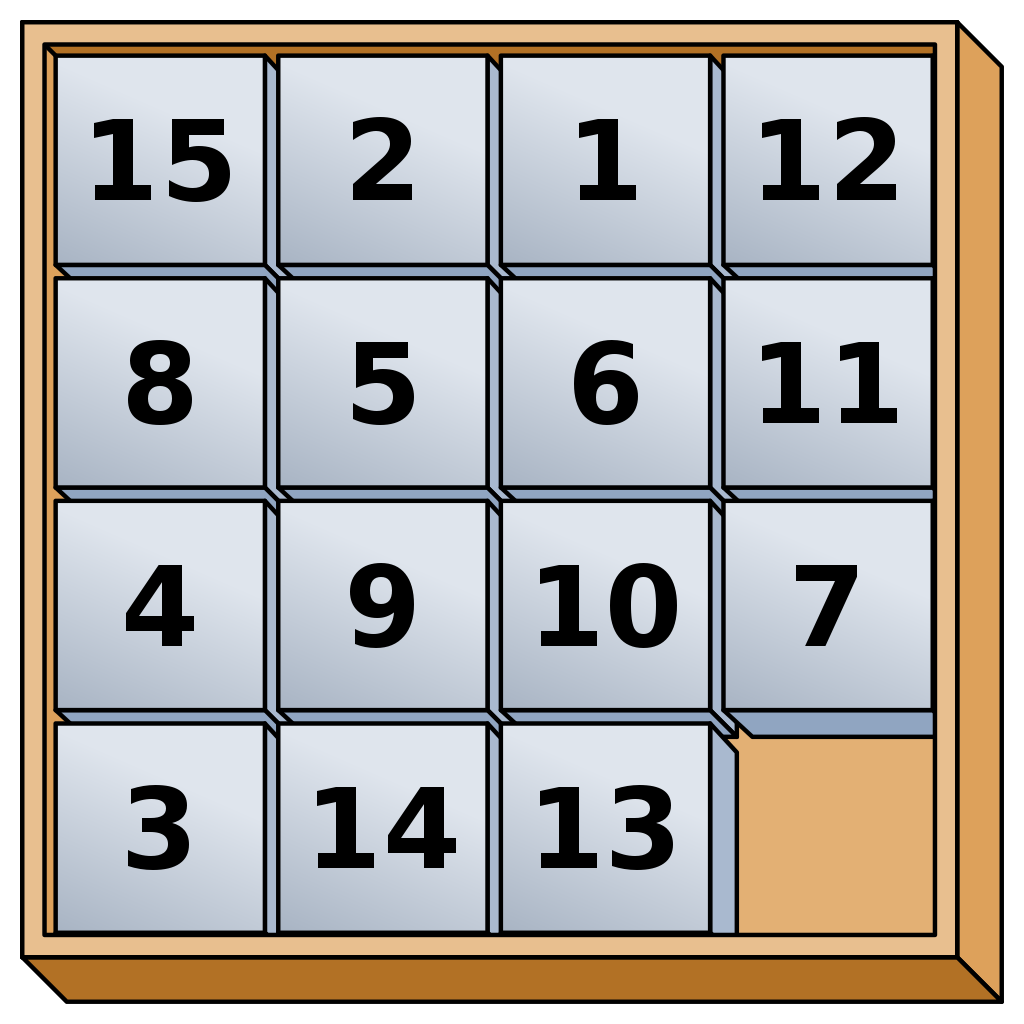
\includegraphics[width=0.25\linewidth]{img/15-puzzle-numbers-scrambled.png}
    }
    \quad\quad\quad\quad
    \subfloat[15-Puzzle mit Zahlen (gelöst)\label{fig-15-puzzle-numbers-solved}]{
      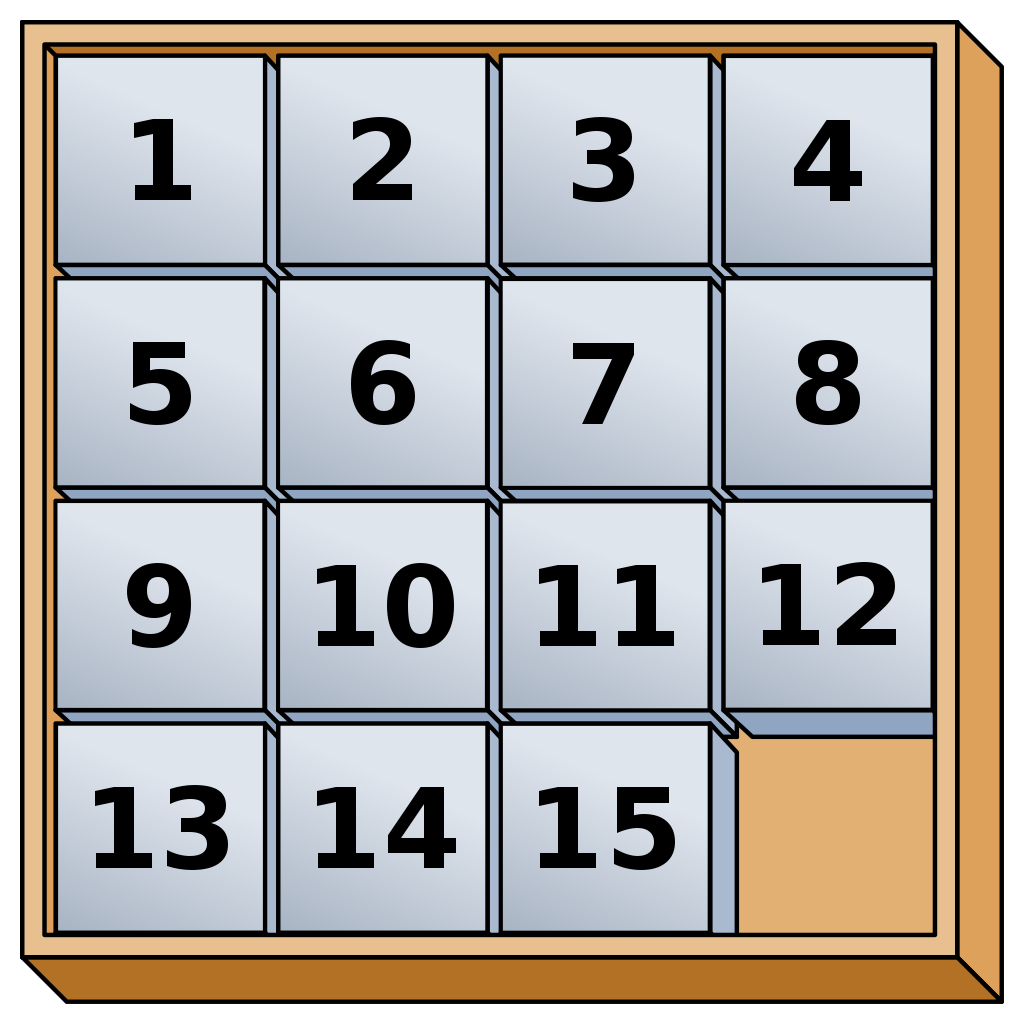
\includegraphics[width=0.25\linewidth]{img/15-puzzle-numbers-solved.png}
    }
    \\
    \subfloat[15-Puzzle mit Bild (gemischt)\label{fig-15-puzzle-image-scrambled}]{
        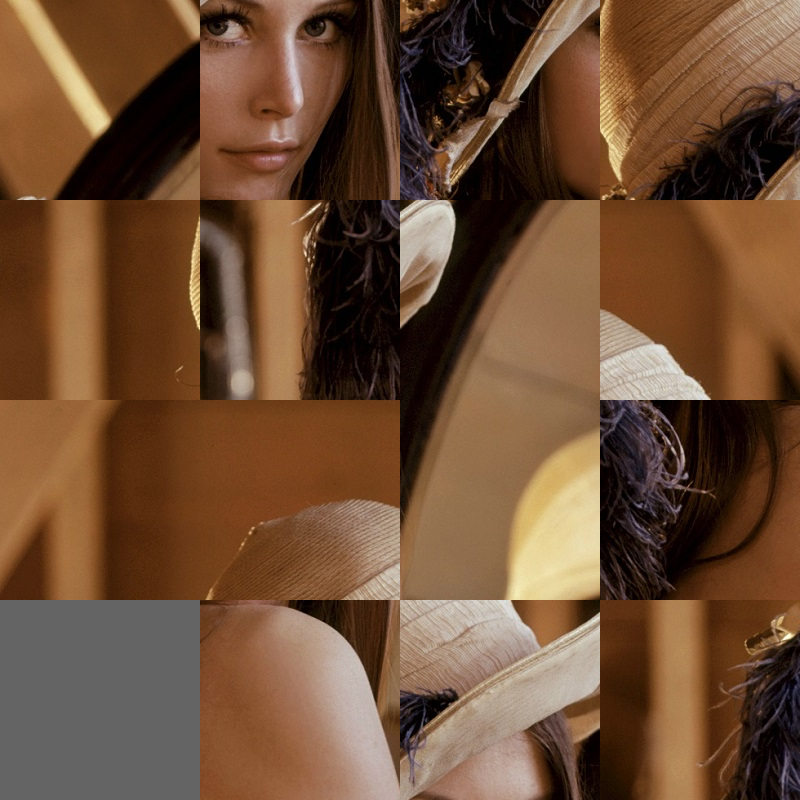
\includegraphics[width=0.25\linewidth]{img/fig-15-puzzle-image-scrambled.png}
    }
    \quad\quad\quad\quad
    \subfloat[15-Puzzle mit Bild (gelöst)\label{fig-15-puzzle-image-solved}]{
        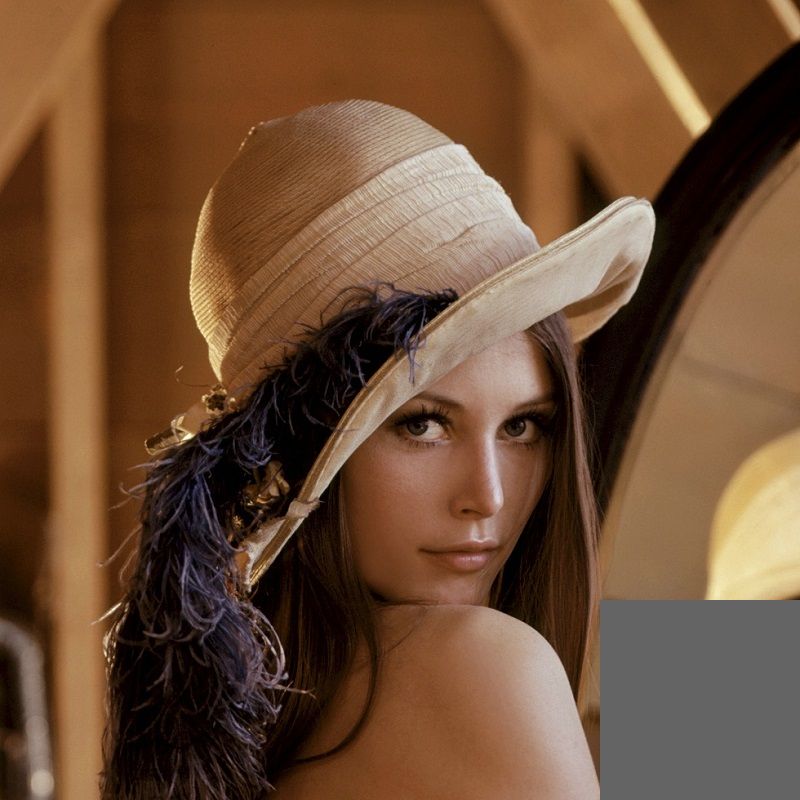
\includegraphics[width=0.25\linewidth]{img/fig-15-puzzle-image-solved.png}
    }
    \caption{Zwei Arten des 15-Puzzle}
    \label{fig-15-puzzle}
\end{figure}
In der Informatik ist das Lösen von Schiebepuzzles ein klassisches Problem der künstlichen Intelligenz und ein übliches Beispielproblem für die Modellierung und Illustration von Suchalgorithmen. Dabei beschränkt sich die meiste Literatur auf das Lösen des klassischen Schiebepuzzles mit Zahlen. Um diese Lösungsverfahren auf ein Schiebepuzzle mit Bild zu übertragen, muss also zuvor seperat das Originalbild rekonstruiert werden.

In dieser Arbeit wird genau solch ein zweischrittiger Ansatz erläutert und analyisert.
\section{Problemstellung und Zielsetzung}
In dieser Arbeit wird das Problem anhand des allgemeinen $N$-Puzzles betrachtet mit $N=m\times n-1$ (für das 15-Puzzle gilt somit $m=n=4$).
\marginpar{$m$: Anzahl der Zeilen}
\marginpar{$n$: Anzahl der Spalten}
Die $N$ Puzzlestücke sind dabei rechteckige Teile eines Bildes. Diese müssen nicht zwingend quadratisch sein, sollten aber alle das gleiche Seitenverhältnis aufweisen, damit diese als Teil eines Schiebepuzzles auch wirklich alle verschiebbar sind und sich somit in den Zustand eines Schiebepuzzles zusammensetzen lassen.

Die Position des leeren Feldes ist dabei nicht zwingend fest (so wie in \ref{fig-15-puzzle} z.\,B. immer unten-rechts) und kann variieren. Diese Position ist außerdem unbekannt und muss damit anhand der Zusammensetzung der restlichen $N$ Puzzleteilen und den bekannten Dimensionen des Puzzles ausgemacht werden.

Außerdem wird noch eine $m\times n$ Anordnung der $N$ Puzzlestücke (und dem leeren Feld) als Anfangszustand vorgegeben.

Folgende Fragen sollen dann (in dieser Reihenfolge) beantwortet werden:
\begin{enumerate}
    \item Wie sah das originale Bild aus und wo befindet sich das leere Feld im Ausgangsbild (wo fehlt also ein Stück des Bildes)?
    \item Ist das Puzzle lösbar, lässt sich also der gegebene Anfangszustand unter einer endlichen Sequenz von legalen Zügen (also ausschließlich durch das hin- und herschieben von Puzzlestücken) in den zuvor ermittelten Endzustand transformieren?
    \item Wie viele Schritte (Verschiebungen) sind mindestens nötig, um das Puzzle zu lösen und wie sieht ein optimaler Lösungsweg (ein Lösungsweg mit der kleinstmöglichen Anzahl an Verschiebungen) aus?
\end{enumerate}
Dazu wird ein vollautomatischer Schiebepuzzlelöser programmiert, der genau diese Schritte abarbeitet und am Ende bei einer gefundenen (optimalen) Lösung das Ergebnis dem Benutzer präsentiert.

Programmiert wird der Puzzlelöser in der Programmiersprache C++. Zur Analyse und Verarbeitung des Bildes wird die Open Source Computer Vision Bibliothek OpenCV verwendet.
\section{Aufbau der Arbeit}
Zunächst werden einige Grundlagen angesprochen, die den Umgang mit OpenCV erläutern und unter anderem aufklären, wie Bilder in OpenCV dargestellt und bearbeitet werden können.

Da zur Rekonstruktion Informationen wie die Kompatibilität (oder auch Ähnlichkeit) zweier Puzzlestücke notwendig ist, werden daraufhin einige Metriken vorgestellt, die diese Information repräsentieren.

Daraufhin wird die Rekonstruktion des Bildes weiter erläutert und ein Greedy Verfahren vorgestellt, welches dieses Problem mithilfe der zuvor berechneten Metriken löst.

Im nächsten Schritt wird das Puzzle mit seinem Anfangs- und Endzustand in ein äquivalentes Schiebepuzzle mit Zahlen übersetzt. Damit werden die nächsten Schritte anhand dem klassischen Zahlenpuzzle (jedoch weiterhin mit beliebigen Dimensionen und beliebigem Anfangs- und Endzustand) gezeigt.

Es wird dann erläutert, wie sich die Lösbarkeit eines Schiebepuzzles bestimmen lässt. Zusätzlich wird geklärt, wie sich zufällige Schiebepuzzle so generieren lassen, dass diese wahlweise immer lösbar oder immer unlösbar sind.

Zum Schluss werden Suchalgorithmen aus der künstlichen Intelligenz vorgestellt, die das eigentliche Lösen des Puzzles übernehmen. Dazu werden sowohl uninformierte Suchalgorithmen, als auch informierte Suchalgorithmen (welche Heuristiken in ihre Suche mit einbeziehen) untersucht und verglichen. An dieser Stelle werden somit auch verschiedene Heuristiken für Schiebepuzzle vorgestellt.
\chapter{OpenCV Grundlagen}
OpenCV (Open Source Computer Vision) ist eine Open Source Programmbibliothek, die mehr als 2500 optimierte Algorithmen aus den Bereichen Bildverarbeitung, maschinelles Sehen und maschinelles Lernen beinhaltet.\cite{opencv} OpenCV steht als freie Software (unter den Bedingungen der BSD-Lizenz) für die Programmiersprachen C++, Java, Python und MATLAB und den Betriebssystemen Windows, Linux, Android und Mac OS zur Verfügung. OpenCV wurde nativ in der Programmiersprache C++ geschrieben und bietet somit Schnittstellen an, die reibungslos mit der C++ Standard Template Library (STL) arbeiten.

OpenCV ist modular aufgebaut und bietet unter anderem folgende wichtige Module an:
\begin{itemize}
    \item \texttt{core} - Dieses Modul definiert einen Großteil der grundlegenden Funktionen und Datenstrukturen von OpenCV (wie z.\,B. die \texttt{cv::Mat}-Klasse beschrieben in \ref{section-mat}).
    \item \texttt{imgproc} - Das Image-Processing Modul implementiert Filter (sowohl lineare Filter als auch nicht lineare Filter), geometrische Bildtransformationen (lineare, linear-affine und perspektivische Transformationen), Histogramme und Methoden zur Konvertierung zwischen verschiedenen Farbräumen.
    \item \texttt{video} - Modul zur Videoanalyse, welches unter anderem Object-Tracking und auch Motion-Estimation Algorithmen implementiert.
    \item \texttt{calib3d} - Implementiert Algorithmen zur Kamerakalibrierung und Elemente zur 3D-Rekonstruktion.
    \item \texttt{features2d} - Bietet Algorithmen zum Erkennen und Matchen von Features in 2D an.
    \item \texttt{objdetect} - Erkennung von Objekten vordefinierter Klassen (z.\,B. Gesichtserkennung)
    \item \texttt{highgui} - Bietet dem Programmierer Möglichkeiten an, simple grafische Benutzungsschnittstellen zu erstellen.
\end{itemize}
\section{Mat - Der OpenCV Bild-Container}\label{section-mat}
Die OpenCV Programmbibliothek war ursprünglich eine Programmbibliothek für die Programmiersprache C. Damit wurden die Datenstrukturen der Bibliothek als C-Structs implementiert, wodurch der Programmierer selber sicherstellen musste, dass der Speicher für diese Datenstrukturen richtig allokiert, deallokiert und gegebenenfalls auch kopiert wird.

Mit der Version OpenCV 2.0 wurde erstmals eine neue C++ Schnittstelle implementiert. Auf Basis der objektorientierten Prinzipien von C++ wie z.\,B. Klassen, Konstruktoren (auch Copy- und Move-Konstruktoren), Destruktor, Resource Acquisition Is Initialization (RAII), Operatorüberladung und Template-Programmierung, somit entstand ein abstrakteres und damit auch einfacheres Interface für den Umgang mit Bildern in OpenCV. Die Klasse \texttt{cv::Mat} ist ein wichtiger Bestandteil dieser Schnittstelle.

Die \texttt{cv::Mat} Klasse stellt eine $n$-dimensionale \textit{dense} Matrix da. Im Gegensatz zu einer \textit{sparse} Matrix (im OpenCV durch die Klasse \texttt{cv::SparseMat} implementiert), welche nur Elemente $\neq0$ speichert, werden bei \texttt{cv::Mat} alle Elemente gespeichert. Die Elemente können sowohl Single-Channel bzw. skalar (z.\,B. Intensität bei Graustufenbildern) oder Multi-Channel bzw. vektorwertig (z.\,B. Intensität einzelner Farbchannel) sein.

Bei $n$-Dimensionen und Dimensionsgrößen $(m_1,\dots,m_n)$ ergeben sich somit $$N=\prod_{k=1}^{n}m_k$$ Elemente, welche intern kontinuierlich in einem $N$-Element großen (eindimensionalem) Array gespeichert sind. Der (nullbasierte) Array-Index $j$ eines Elementes mit den Dimensions-Indizes $(i_1,\dots,i_n)$ lässt sich dann durch folgende rekursive Relation berechnen\cite{opencv2} (mit $j=j_n$): $$j_k=\begin{cases}j_{k-1}\cdot m_k+i_k,&k\neq0\\0&k=0\end{cases}$$.

Im zweidimensionalen Fall ($n=2$) reduziert sich dies zu $j=i_1\cdot m_2+i_2$. Mit $i_1$ als Zeilenindex, $i_2$ als Spaltenindex und der Anzahl an Spalten $m_2$. Somit werden zweidimensionale Matrizen also Zeile-für-Zeile gespeichert, dreidimensionale Matrizen zunächst Ebene-für-Ebene und dann jede Ebene wieder Zeile-für-Zeile.

Dieses Speicherlayout ist üblich für \textit{dense} Arrays und ist kompatibel mit anderen Bibliotheken, die ein solches Speicherlayout voraussetzen. Dazu gehört auch die C++ STL. Diese Kompatibilität ermöglicht es nicht nur, STL-Algorithmen auf die Daten eines \texttt{cv::Mat}-Objektes anzuwenden, sondern es bietet sich auch die Möglichkeit an, selbst allokierte Daten in ein \texttt{cv::Mat}-Objekt zu wrappen und diese Daten dann mit OpenCV spezifischen Methoden zu bearbeiten.

Die \texttt{cv::Mat}-Klasse ist stark an die Matrizen aus MATLAB angelehnt, womit OpenCV die Möglichkeit bietet Matrizen im MATLAB-Style zu initialisieren mit z.\,B. \texttt{cv::Mat::zeros()} um alle Elemente der Matrix mit $0$ zu initialisieren, \texttt{cv::Mat::ones()} um alle Elemente mit $1$ zu initialisieren und \texttt{cv::Mat::eye()} zur Konstruktion einer Einheitsmatrix.

Die Datenstrukturen von OpenCV (und damit auch \texttt{cv::Mat}) implementieren bereits die nötigen Maßnahmen zur Speicherverwaltung, womit dies nicht vom Programmierer übernommen werden muss. Dabei sei jedoch zu beachten, dass \texttt{cv::Mat} jedoch nicht wie die meisten C++ Datenstrukturen mit dynamischem Speicher (z.\,B. \texttt{std::vector}) implementiert ist.

Ein \texttt{std::vector} wird beim Kopieren (entweder beim Initialisieren eines anderen Vectors mit dem Kopier-Konstruktor oder durch den Assignment-Operator) komplett kopiert und bekommt seinen eigenen Speicher, der nun die gleichen Daten enthält wie der Originalvector. Es wird kein Speicher zwischen den beiden Objekten geteilt und jedes Objekt ist für seinen eigenen Speicher zuständig. Um die lineare Laufzeit beim Kopieren zu umgehen, wo diese nicht nötig ist, wird Referenzübergabe verwendet. Auch das Kopieren von temporären Objekten, sogenannten rvalues (da solche Objekte bei nur links vom Assignment-Operator stehen dürfen), lässt sich seit C++11 mithilfe von Move-Semantiken in konstanter Zeit durchführen.

Im Gegensatz dazu teilen \texttt{cv::Mat}-Objekte ihre Resourcen (den darunterliegenden Speicher) gegebenenfalls mit anderen \texttt{cv::Mat}-Objekten. Dazu implementiert \texttt{cv::Mat} Reference-Counting und arbeitet somit ähnlich wie der Smart-Pointer \texttt{std::shared\_ptr} der C++11-Library oder auch wie Objekte in anderen Programmiersprachen wie Java oder C\#. Dies hat zu Folge, dass die Destruktoren von \texttt{cv::Mat}-Objekten zunächst die Reference-Count dektrementieren und den Speicher erst dann wieder freigeben, wenn die Reference-Count mit dem destrukten des letzten Objektes auf $0$ gefallen ist. Der Vorteil hierbei ist, dass das Kopieren einer Matrix genau genommen die Daten nicht wirklich kopiert, sondern lediglich den Matrix-Header (mit Metadaten wie Dimensionsgrößen und der Adresse zum Speicher der Daten) übernimmt und den Reference-Counter inkrementiert. Das Kopieren einer Matrix ist also unabhängig von der Größe der Matrix und somit konstant. Um eine Matrix vollständig zu kopieren bietet OpenCV in der \texttt{cv::Mat}-Klasse die Methode \texttt{cv::Mat::clone()} an.

Die Kopiersemantik von \texttt{cv::Mat} ist dann von wichtiger Bedeutung, wenn es gilt, einen Teilbereich einer Matrix zu extrahieren oder zu ändern. Solche Bereiche werden als Region of Interest (ROI) bezeichnet und können eine oder mehrere Zeilen, eine oder mehrere Spalten, eine Diagonale oder ein rechteckiger Bereich aus der Matrix sein. Diese Operationen sind weiterhin alle $\Theta(1)$, da lediglich ein neuer Matrix-Header erstellt werden muss und die eigentlichen Elemente der Matrix nicht kopiert werden, sondern nur referenziert werden. Damit wirken sich Änderungen der Daten in einer Matrix also auch implizit auf alle anderen Matrizen aus, die diese Daten referenzieren.

\section{Saturate-Casting}\label{section-sat}
Die einzelnen Pixels eines Bildes sind in OpenCV Elemente einer zweidimensionalen \texttt{cv::Mat}. Ob diese Elemente skalar oder vektorwertig sind hängt vom gewählten Farbraum ab. Die Wertebereiche der einzelnen Channel eines Elementes hängen wiederum vom gewählten Datentyp ab (vgl. \ref{section-pixeltypes}). Dabei werden oftmals 8- oder 16-bit (signed oder unsigned) per Channel gewählt. Für unsigned 8-bit (Datentyp \texttt{cv::uchar} in OpenCV) stehen damit nur ganzzahlige Werte aus dem (halboffenen) Intervall $[0, 256)$ zu Verfügung. Viele Operationen auf Bildern (z.\,B. das Interpolieren von Bildern oder das Konvertieren zwischen verschiedenen Farbräumen) können Werte ausserhalb dieses Intervalles erzeugen. Anstatt jedoch nur die niedrigsten 8 Bits des Ergebnisses zu verwenden (was in einem Bild unmittelbar zu sichtbaren Artifakten führt), bietet OpenCV einen \texttt{cv::saturate\_cast<>()} an, welcher den berechneten Wert auf den nächsten Wert im zugelassenen Wertebereich vom Datentyp abbildet. Dazu wird der Wert zunächst gerundet. Falls der gerundet Wert ausserhalb des gültigen Wertebereiches liegt, wird dieser auf den nächsten Wert gültigen Wert gesetzt (jeweils auf das Minimum oder Maximum der Intervalls, je nachdem ob der Wert auf dem Zahlenstrahl links oder rechts vom Intervall liegt). Der letzte Schritt wird auch als \textit{Clamping} bezeichnet. Eine mögliche Implementation\cite{opencv3} für einen 8-bit Channel mit einem berechneten Wert $v$ ist $$v'=\min\{\max\{\lfloor v+0.5\rfloor,0\},255\}$$.
\section{Datentypen für Pixel}\label{section-pixeltypes}
Anstatt die Wahl des Datentyps für Pixel generisch zu halten (mithilfe von C++ Templates), gibt OpenCV eine feste limitierte Menge an primitiven Datentypen für Matrizen vor.\cite{opencv3} Der Grund dafür ist, dass große Template Klassen die Compilezeit und die größe des Codes stark erhöhen. Außerdem lassen sich Templates nur schlecht in Definition und Implementation aufteilen (wie es sonst mit Header- und Source-Dateien üblich ist). Des Weiteren besitzen die anderen Sprachen, welche von OpenCV unterstützt werden (Python, MATLAB und Java), keine oder nur begrenzte Sprachkonstrukte, welche die Implementation von Templates ermöglichen würde. Stattdessen basiert die aktuelle OpenCV Implementation hauptsächlich auf Polymorphismus. In C++ stehen aus Performancegründen (um die dynamische Laufzeitbindung von polymorphen Methoden zu vermeiden) jedoch einzelne Template Klassen, Methoden und Funktionen zur Verfügung (dazu gehört auch der \texttt{cv::saturate\_cast<>()}.

In OpenCV stehen folgende primitive skalare Datentypen für Matrizen zur Verfügung:
\begin{itemize}
    \item 8-bit unsigned Integer - \texttt{cv::uchar}
    \item 8-bit signed Integer - \texttt{cv::schar}
    \item 16-bit unsigned Integer - \texttt{cv::ushort}
    \item 16-bit signed Integer - \texttt{cv::short}
    \item 32-bit signed Integer - \texttt{cv::int}
    \item 32-bit floating-point Zahl - \texttt{cv::float}
    \item 64-bit floating-point Zahl - \texttt{cv::double}
\end{itemize}
Für Multi-Channel Matrizen wird vorausgesetzt, dass jeder Channel den gleichen Datentyp besitzt (außerdem muss dieser natürlich einer der oben aufgeführten Datentypen sein). Des Weiteren ist die maximale Anzahl an möglichen Channels per Matrixelement auf $512$ begrenzt.

Die oben aufgeführten Typen werden zwar als Template-Argument für einzelne Funktionen von OpenCV verwendet (z.\,B. für den bereits erwähnten \texttt{cv::saturate\_cast<>()}), spezifizieren aber nicht den Datentyp für Matrixelemente (da \texttt{cv::Mat} schließlich nicht generisch ist). Stattdessen besitzen diese Klassen dann einen weiteren Parameter im Konstruktur, mit dem der Datentyp angegeben werden kann. Für die skalaren Typen gilt dabei folgende Enumeration:
\begin{lstlisting}[numbers=none,frame=none]
enum {
    CV_8U  = 0,
    CV_8S  = 1,
    CV_16U = 2,
    CV_16S = 3,
    CV_32S = 4,
    CV_32F = 5,
    CV_64F = 6
};
\end{lstlisting}
Die Namen für Multi-Channel Konstanten mit $k=1\dots4$ Channels entsprechen dem Namen des Datentyps eines Channels (entsprechend der obigen Enumeration), gefolgt von einem \texttt{C}$k$. Ein Drei-Channel Array vom Typen 16-bit unsigned Integer entspricht also der Konstanten \texttt{CV\_16UC3}.

Um einen Matrix mit mehr als vier Channels zu initialisieren oder falls die Anzahl der Channel bei der Compilezeit unbekannt ist, lassen sich die Makros \texttt{CV\_U8C(n)} bis \texttt{CV\_64FC(n)} verwenden. Genau genommen generieren diese Makros lediglich eine numerische Konstante, die intern eine Kombination von Datentyp und Anzahl an Channels identifiziert. Dazu wird die Konstante des Datentyps (entsprechend den Werten in der Enumeration) in die niedrigsten 3 Bits gehschrieben und die Anzahl der Channel dekrementiert (da $0$ Channel sowieso nicht zugelassen sind, lässt sich dadurch eine Möglichkeit mehr darstellen) und in die restlichen Bits geschrieben. Dementsprechend sind für die Anzahl der Channels standardmäßig $\log_2(512)=9$ Bits vorgesehen. Die Berechnung der numerischen Konstante eines Multi-Channel Datentyps ist in OpenCV mit dem Makro \texttt{CV\_MAKETYPE(depth, cn)} implementiert, dabei entspricht \texttt{depth} der numerischen Konstante des Datentyps entsprechend der Enumeration und \texttt{cn} die Anzahl der Channel (\texttt{cn > 0}). Eine mögliche Implementation nach \cite{opencv4} dieses Makros sieht folgendermaßen aus:
\begin{lstlisting}[numbers=none,frame=none]
#define CV_MAKETYPE(depth, cn) (((depth) & 7) | (((cn)-1) << 3))
\end{lstlisting}
Damit ergeben sich viele equivalente Möglichkeiten, den Datentyp einer Matrix festzulegen. So gilt z.\,B. \texttt{2 == CV\_16U == CV\_16UC1 == CV\_16UC(1) == CV\_MAKETYPE(CV\_16U, 1) == (2 \& 7) | ((1 - 1) << 3) == 2}, was mit der ursprünglichen Definition aus der Enumeration übereinstimmt.

Was genau die Werte eines einzelnen Elementes darstellen, hängt vom Farbraum des Bildes ab. Beim Einlesen eines Bildes in OpenCV mit der Funktion \texttt{cv::imread()} lässt sich als Parameter mit angeben, ob dieses Bild als Graustufenbild gelesen werden soll (\texttt{IMREAD\_GRAYSCALE}) oder als Farbbild (\texttt{IMREAD\_COLOR}). Als Rückgabewert liefert die Funktion eine (zweidimensionale) Matrix in den Dimensionen des ursprünglichen Bildes. Jedes Element der Matrix stellt einen Bildpunkt des Bildes in dem entsprechenden Farbraum (wird dieser nicht explizit angegeben, so wird implizit der Parameter \texttt{IMREAD\_COLOR} verwendet) dar. Bei Graustufenbildern bestehen diese Elemente nur aus einem Channel (der Intensität dieses Bildpunktes), während bei Farbbildern das BGR-Format verwendet wird. Hierbei steht der Wert jedes Channels (von insgesamt drei) für die Intensität der entsprechenden Farbe (\textbf{B}lau, \textbf{G}rün oder \textbf{R}ot) im Bildpunkt. Das BGR-Format ist abgesehen von der Reihenfolge der Farbchannel identisch zu dem bekannten RGB-Format.

Um Bilder zwischen verschiedenen Farbräumen zu konvertieren lässt sich die OpenCV Funktion \texttt{cv::cvtColor()} verwenden. Es lässt sich als Parameter angeben, welche Art von Konvertieren stattfinden soll (z.\,B. \texttt{COLOR\_BGR2GRAY}).\cite{opencv5}

\section{Beispiel: Verwendung von Matrizen und Region of Interests}
Es folgt ein Codeausschnitt, der die Eigenschaften von \texttt{Mat} nach Abschnitt \ref{section-mat} nochmals aufzeigt.
\begin{lstlisting}[caption=Verwendung von Mat und ROI, label=lst-mat-example]
cv::Mat a(256, 256, CV_8UC3, cv::Scalar(100, 100, 100));
cv::Mat b = a;
cv::Mat c = a.clone();

a.colRange(50, 80).setTo(cv::Scalar(255, 0, 0));
b.diag().setTo(cv::Scalar(0, 255, 0));
c({ 0, 20 }, { 0, 20 }).setTo(cv::Scalar(0, 0, 255));

cv::namedWindow("a");
cv::imshow("a", a);

cv::namedWindow("b");
cv::imshow("b", b);

cv::namedWindow("c");
cv::imshow("c", c);

cv::waitKey();
cv::destroyAllWindows();
\end{lstlisting}
Im Beispiel wird zunächst eine zweidimensionale $256\times256$ Matrix \texttt{a} vom Typen \texttt{CV\_8UC3} angelegt und jeder der drei 8-bit Farbchannel mit $100$ initialisiert, was im BGR Farbraum einem Grauton entspricht. Die Matrix benötigt somit insgesamt exakt $192$ Kibibyte, um die Farbwerte der Pixel zu speichern (mit Headerdaten ist diese natürlich noch größer). Die Initialisierung von \texttt{b} in der darauffolgenden Zeile führt wie in \ref{section-mat} beschrieben lediglich dazu, dass die Headerdaten von \texttt{a} übernommen werden. Damit befindet sich weiterhin nur ein (komplett graues) Bild im Speicher, welches jedoch von zwei verschiedenen \texttt{Mat}-Objekten (\texttt{a} und \texttt{b}) referenziert wird. Die Initialisierung von Matrix \texttt{c} entspricht hingegen einer tiefen Kopie der Matrix \texttt{a}, wodurch nun zwei (gleiche) Bilder im Speicher liegen. Diese Operation muss den kompletten Speicher von \texttt{a} kopieren, was zu einem linearen Laufzeitverhalten fürt.

Die nächsten Zeilen zeigen, wie ROIs in OpenCV verwendet werden können, um Teilbereiche einer Matrix zu extrahieren und zu bearbeiten. Zeile 5 erstellt eine temporäre Matrix, welche auf den gleichen Speicherbereich von \texttt{a} zeigt, die Headerdaten jedoch so definiert werden, dass diese Matrix nur einen Teilbereich von \texttt{a} schreiben und lesen kann. Als ROI werden hier die Spaltenvektoren von \texttt{a} mit Spaltenindizes (nullbasiert) aus dem Intervall $[50,80)$ genommen. Damit ergibt sich eine temporäre $256\times30$ Matrix. Alle Elemente dieser Matrix werden daraufhin blau gefärbt, wodurch natürlich auch die entsprechenden Spalten in \texttt{a} betroffen sind und damit auch implizit das Bild der Matrix \texttt{b} verändert wird (was schließlich das Bild aus der Matrix \texttt{a} ist). Zeile 6 färbt die Hauptdiagonale von \texttt{b} $\{b_{ij}:(i,j)\in[0,256)^2\land i=j\}$ grün (was wiederum die Matrix \texttt{a} mit betrifft). Die Matrix \texttt{c} hat zu diesem Zeitpunkt immer noch ein rein graues Bild. Zeile 7 zeigt, wie man eine beliebige rechteckige ROI aus einer Matrix extrahiert. Im Beispiel wird eine $20\times20$ ROI erstellt mit den Matrixelementen $\{c_{ij}:0\leq i,j<20\}$, welche daraufhin rot gefärbt werden. Diese Operation betrifft ausschließlich die Matrix \texttt{c}; \texttt{a} und \texttt{b} werden nicht verändert.

Die nächsten Zeilen stellen den Inhalt der Matrizen dar. Die Ausgabe ist in \ref{fig-opencv-mat} dargestellt. Wie erwartet zeigen die Matrizen \texttt{a} und \texttt{b} das selbe Bild.
\begin{figure}[H]
    \centering
    \subfloat[\label{fig-opencv-mat-a}]{
      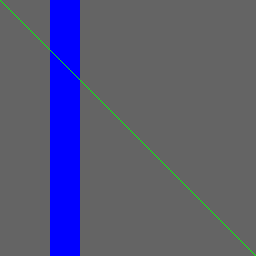
\includegraphics[width=0.25\linewidth]{img/a.png}
    }
    \quad\quad
    \subfloat[\label{fig-opencv-mat-b}]{
      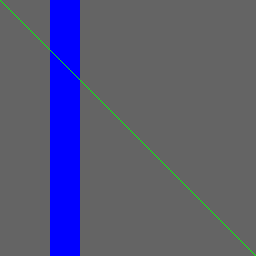
\includegraphics[width=0.25\linewidth]{img/b.png}
    }
    \quad\quad
    \subfloat[\label{fig-opencv-mat-c}]{
      
\includegraphics[width=0.25\linewidth]{img/c.png}
    }
    \caption{Ausgabe vom Mat und ROI Beispiel}
    \label{fig-opencv-mat}
\end{figure}
\section{Transformation von Bildern}
Um bekannte lineare Transformationen (Skalierung, Rotation, Scherung) und affine Transformationen (lineare Transformationen mit einer Translationskomponente) auf Bildern anzuwenden, bietet OpenCV die Funktion \texttt{cv::warpAffine()} an. Neben dem Ausgangsbild, auf welches die Transformation angewendet werden soll, und einem Zielbild, welches das Ergebnis der Transformation halten soll, übernimmt diese Funktion noch eine $2\times3$ Transformationsmatrix.

Eine affine Transformation $T:\mathbb{R}^2\rightarrow\mathbb{R}^2$ bildet einen Vektor $\vec{x}=\begin{bmatrix}x\\y\end{bmatrix}\in\mathbb{R}^2$ auf einen Vektor $T(\vec{x})\in\mathbb{R}^2$ ab. Eine solche Transformation hat die Form
\begin{gather*}
    T(\vec{x})=\mathbf{A}\vec{x}+\vec{b}
\end{gather*}
mit $\mathbf{A}=\begin{bmatrix}a_{11}&a_{12}\\a_{21}&a_{22}\end{bmatrix}\in\mathbb{R}^{2\times2}$ und dem Translationsvektor $\vec{b}\in\mathbb{R}^2$.

Für $\vec{b}=\vec{0}$ ist $T$ eine lineare Transformation. Eine solche Transformation erfüllt folgende Bedingung ($T$ ist homogen und additiv): $T(\alpha\vec{u}+\vec{v})=\alpha T(\vec{u})+T(\vec{v})$ für ein Skalar $\alpha\in\mathbb{R}$ und zwei Vektoren $\vec{u},\vec{v}\in\mathbb{R}^2$. Eine Implikation dieser Bedingung ist, dass der Nullvektor stets auf sich selber abgebildet wird: $T(\vec{0})=T(0\cdot\vec{e}_1+0\cdot\vec{e}_2)=0\cdot T(\vec{e}_1)+0\cdot T(\vec{e}_2)=\vec{0}+\vec{0}=\vec{0}$.

Wird $\vec{x}$ in homogenen Koordinaten betrachtet ($\vec{x}=\begin{bmatrix}x&y&1\end{bmatrix}^\mathsf{T}$), so lässt sich eine Matrix $\mathbf{M}$ zur Transformation $T$ angeben.
\begin{align*}
    T(\vec{x})&=\mathbf{A}\vec{x}+\vec{b}\\
    T(\vec{x})&=\begin{bmatrix}a_{11}&a_{12}\\a_{21}&a_{22}\end{bmatrix}\cdot\begin{bmatrix}x\\y\end{bmatrix}+\begin{bmatrix}b_1\\b_2\end{bmatrix}\\
    T(\vec{x})&=x\cdot\begin{bmatrix}a_{11}\\a_{21}\end{bmatrix}+y\cdot\begin{bmatrix}a_{12}\\a_{22}\end{bmatrix}+1\cdot\begin{bmatrix}b_1\\b_2\end{bmatrix}\\
    T(\vec{x})&=\underbrace{\begin{bmatrix}a_{11}&a_{12}&b_1\\a_{21}&a_{22}&b_2\end{bmatrix}}_{\eqqcolon\mathbf{M}\in\mathbb{R}^{2\times3}}\cdot\begin{bmatrix}x\\y\\1\end{bmatrix}
\end{align*}
Die Funktion \texttt{cv::warpAffine()} transformiert das Originalbild dann so, dass $$dst(\vec{x})=src(T^{-1}(\vec{x}))$$.\cite{opencv6}

Damit arbeitet die Funktion also mit der inversen Transformation, welche sich mit der Funktion \texttt{cv::invertAffineTransform()} berechnen lässt. Standardmäßig wird dies bereits von \texttt{cv::warpAffine()} übernommen. Liegt die Transformation jedoch schon invertiert vor, lässt sich diese auch an die Funktion übergeben. Das Setzen von dem \texttt{WARP\_INVERSE\_MAP}-Flag bewirkt dann, dass das Invertieren der Transformation übersprungen wird.

Um Beispielsweise das Bild um 90° (gegen den Uhrzeigersinn) um den Bildmittelpunkt zu rotieren, lässt sich eine Transformation als Komposition von Translation und Rotation angeben. Dabei ist zu beachten, dass der Ursprung des Koordinatensystems sich an der linkeren oberen Ecke des Bildes befindet. Die x-Achse zeigt nach rechts und die y-Achse nach unten. Bei einem Bild mit Breite $w$ und Höhe $h$ gilt $(x,y)\in[0,w)\times[0,h)$ womit sich der Bildmittelpunkt bei $(\frac{w-1}{2},\frac{h-1}{2})$ befindet.

Die entsprechende Transformationsmatrix $\mathbf{M}$ lautet dann $$\mathbf{M}=\begin{bmatrix}1&0&\frac{w-1}{2}\\0&1&\frac{h-1}{2}\end{bmatrix}\cdot\underbrace{\begin{bmatrix}0&1&0\\-1&0&0\\0&0&1\end{bmatrix}}_{Rotation}\cdot\begin{bmatrix}1&0&-\frac{w-1}{2}\\0&1&-\frac{h-1}{2}\\0&0&1\end{bmatrix}$$.

Die homogene Komponente wird bis zur letzten Transformation erhalten, um die Komposition von affinen und linearen Transformationen zu ermöglichen. Da \texttt{cv::warpAffine()} jedoch eine $2\times3$ Matrix benötigt, wird die letzte Matrix auch als $2\times3$ Matrix angegeben.
\begin{figure}[H]
    \centering
    \subfloat[src\label{fig-opencv-affine-1-src}]{
      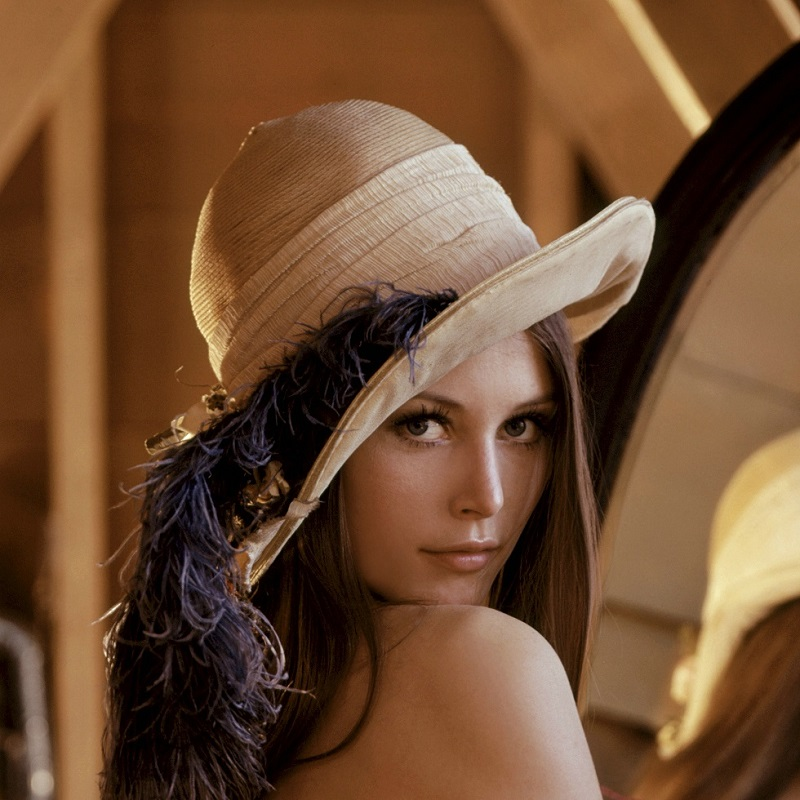
\includegraphics[width=0.25\linewidth]{img/affine_1_src.png}
    }
    \quad\quad\quad\quad
    \subfloat[dst\label{fig-opencv-affine-1-dst}]{
      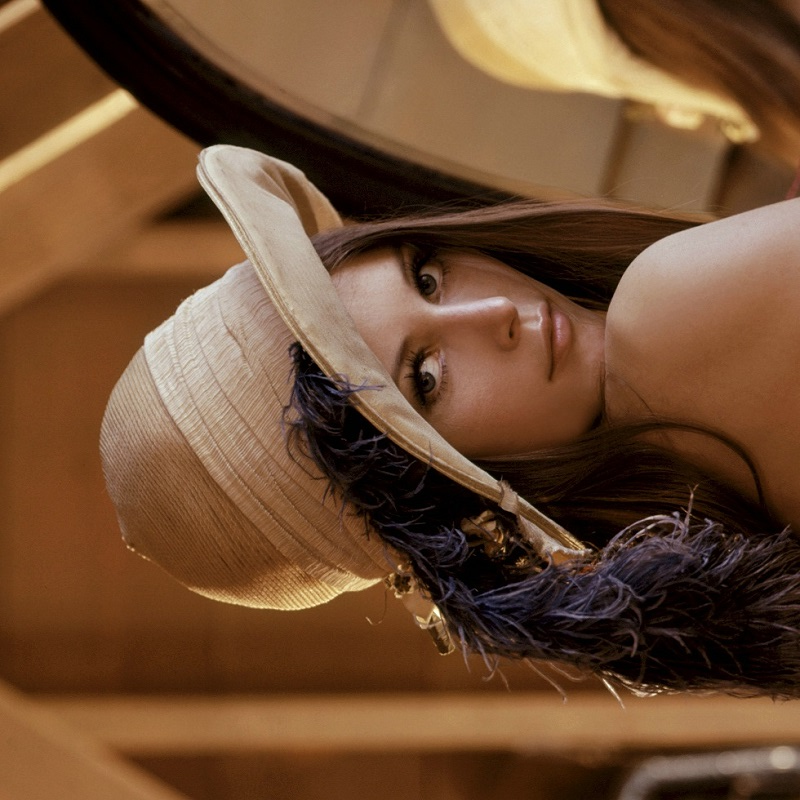
\includegraphics[width=0.25\linewidth]{img/affine_1_dst.png}
    }
    \caption{Rotation als affine Transformation}
    \label{fig-opencv-affine-1}
\end{figure}
Um die entsprechende Transformationsmatrix einer beliebigen Rotation direkt zu bekommen, bietet OpenCV die Funktion \texttt{cv::getRotationMatrix2D()} an, welche neben dem Rotationswinkel (gemessen in Grad und gegen dem Uhrzeigersinn) auch einen Punkt übernimmt, um den rotiert werden soll.

Da eine affine Transformation Dreiecke auf Dreiecke abbildet, lässt sich eine eindeutige affine Transformation finden, welche eine geordnete Menge von drei nicht-kollinearen Punkten auf eine andere Menge dieser Art abbildet.

OpenCV bietet dafür die Funktion \texttt{cv::getAffineTransform()} an. Diese übernimmt drei Punkte $(x_i,y_i)$, welche auf drei andere Punkte $(x_i^\prime,y_i^\prime)$ abgebildet werden sollen ($1\leq i\leq3$). Als Ergebnis liefert diese Funktion eine $2\times3$ Transformationsmatrix $\mathbf{M}$. Dabei ist $\mathbf{M}$ genau die Matrix der affinen Transformation, für die 
\begin{align}
\begin{bmatrix}x_i^\prime\\y_i^\prime\end{bmatrix}=\mathbf{M}\cdot\begin{bmatrix}x_i\\y_i\\1\end{bmatrix},1\leq i\leq3 \label{eq1}
\end{align}.\cite{opencv6}

Mit $$\mathbf{M}=\begin{bmatrix}m_{11}&m_{12}&m_{13}\\m_{21}&m_{22}&m_{23}\end{bmatrix}$$ wird dann intern von der Funktion ein $6\times6$ Gleichungssystem gelöst, um die Koeffizienten von $\mathbf{M}$ herauszufinden. Das Gleichungssystem lautet $$\begin{bmatrix}x_1&y_1&1&0&0&0\\x_2&y_2&1&0&0&0\\x_3&y_3&1&0&0&0\\0&0&0&x_1&y_1&1\\0&0&0&x_2&y_2&1\\0&0&0&x_3&y_3&1\end{bmatrix}\cdot\begin{bmatrix}m_{11}\\m_{12}\\m_{13}\\m_{21}\\m_{22}\\m_{23}\\\end{bmatrix}=\begin{bmatrix}x_1^\prime\\x_2^\prime\\x_3^\prime\\y_1^\prime\\y_2^\prime\\y_3^\prime\\\end{bmatrix}$$.

Alternativ dazu lassen sich auch zwei Matrizen $\mathbf{A},\mathbf{B}$ definieren mit $$\mathbf{A}=\begin{bmatrix}x_1&x_2&x_3\\y_1&y_2&y_3\\1&1&1\end{bmatrix},\mathbf{B}=\begin{bmatrix}x_1^\prime&x_2^\prime&x_3^\prime\\y_1^\prime&y_2^\prime&y_3^\prime\end{bmatrix}$$.

Die Matrix $\mathbf{A}$ bildet die drei Standardbasisvektoren des $\mathbb{R}^3$ ($\vec{e}_1,\vec{e}_2,\vec{e}_3$) auf die drei Vertices des Dreiecks ab (in homogenen Koordinaten). Es gilt also $\begin{bmatrix}x_i&y_i&1\end{bmatrix}^\mathsf{T}=\mathbf{A}\vec{e}_i,1\leq i\leq3$. Allgemein werden alle Vektoren $\begin{bmatrix}\alpha&\beta&\gamma\end{bmatrix}^\mathsf{T}$ mit $\alpha+\beta+\gamma=1$ auf einen Vektor in der Ebene des Dreiecks (also einen Vektor mit $1$ als homogene Komponente) abgebildet. Gilt außerdem noch $\alpha,\beta,\gamma\geq0$, dann ist dies sogar ein Vektor im Dreieck.

Die Matrix $\mathbf{B}$ hat ähnliche Eigenschaften wie $\mathbf{A}$. Hier wurden lediglich die Vertices des zweiten Dreiecks als Spaltenvektoren der Matrix verwendet. Außerdem fehlt hier jeweils die homogene Komponente in den Spaltenvektoren. Dadurch ist der Ergebnisvektor direkt ein Vektor im $\mathbb{R}^2$ (ohne homogene Komponente).

Damit lässt sich $\mathbf{M}$ nun folgendermaßen als Komposition dieser beiden Matrizen darstellen:$$\mathbf{M}=\mathbf{B}\cdot\mathbf{A}^{-1}$$.

Mit $$\begin{bmatrix}x_i&y_i&1\end{bmatrix}\xmapsto{\mathbf{A}^{-1}}\vec{e}_i\xmapsto{\mathbf{B}}\begin{bmatrix}x_i^\prime&y_i^\prime\end{bmatrix}$$ ist dies nach \ref{eq1} genau die gesuchte Matrix für die Transformation.

Die folgende Abbildung zeigt das Ergebnis einer solchen Transformation. Im Bild mit der Breite $w$ und Höhe $h$ wird das Dreieck mit den Vertices $(0,0),(w-1,0),(0,h-1)$ auf das Dreieck mit den Vertices $(\frac{w-1}{2},\frac{h-1}{2}),(0,0),(w-1,0)$ abgebildet.
\begin{figure}[H]
    \centering
    \subfloat[src\label{fig-opencv-affine-2-src}]{
        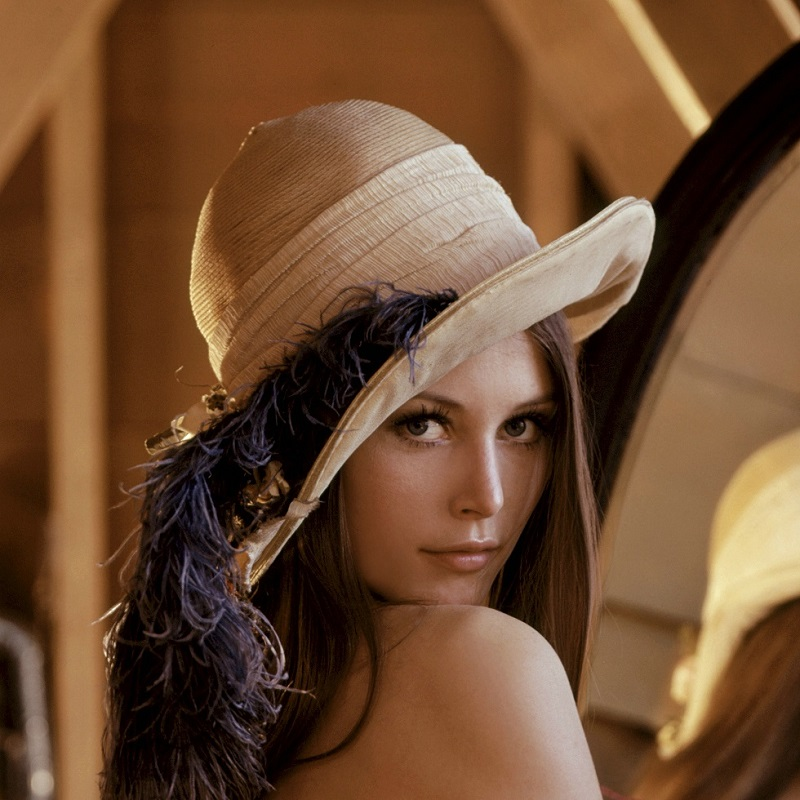
\includegraphics[width=0.25\linewidth]{img/affine_2_src.png}
    }
    \quad\quad\quad\quad
    \subfloat[dst\label{fig-opencv-affine-2-dst}]{
        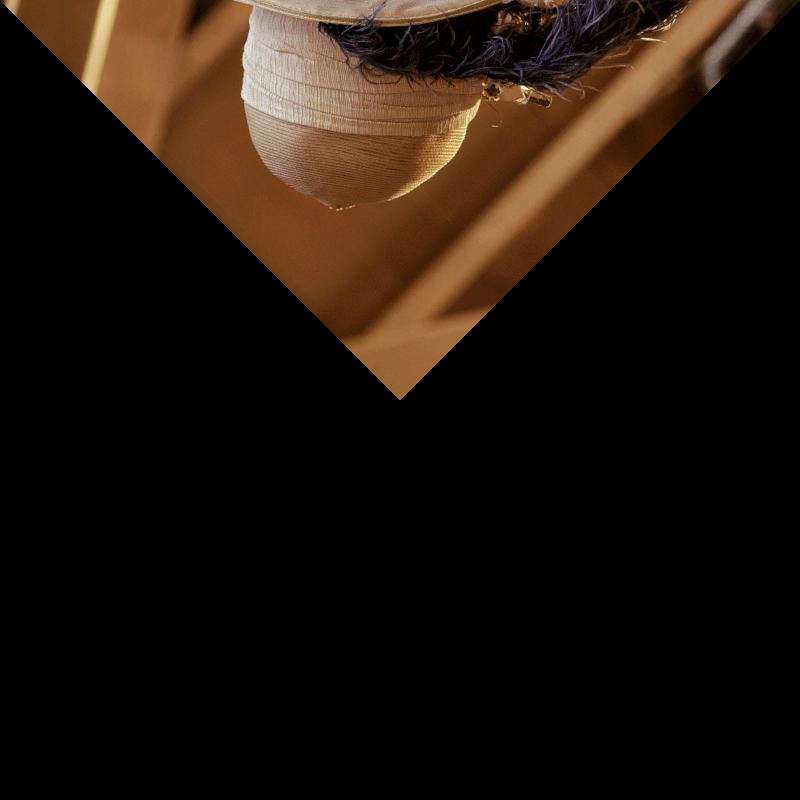
\includegraphics[width=0.25\linewidth]{img/affine_2_dst.png}
    }
    \caption{Abbildung zweier Dreiecke als affine Transformation}
    \label{fig-opencv-affine-2}
\end{figure}
Um die Abbildung zwischen zwei allgemeinen (konvexen) Vierecken darzustellen, muss eine perspektivische Transformation gewählt werden. Schließlich bildet eine affine Transformation parallele Linien wieder auf parallele Linien ab, womit Parallelogramme stets auf Parallelogramme abgebildet werden.

Eine solche perspektivische Transformation lässt sich durch eine $3\times3$ Matrix $\mathbf{P}$ darstellen, welche vier Punkte auf vier andere Punkte abbildet (genau genommen auf ein Vielfaches dieser Punkte), sodass: $$\begin{bmatrix}\lambda_i x_i^\prime\\\lambda_i y_i^\prime\\\lambda_i\end{bmatrix}=\underbrace{\begin{bmatrix}p_{11}&p_{12}&p_{13}\\p_{21}&p_{22}&p_{23}\\p_{31}&p_{32}&p_{33}\end{bmatrix}}_{\mathbf{P}}\cdot\begin{bmatrix}x_i\\y_i\\1\end{bmatrix},1\leq i\leq4$$.

In OpenCV lässt sich diese Matrix mit der Funktion \texttt{cv::getPerspectiveTransform()} finden. Die Funktion \texttt{cv::warpPerspective()} übernimmt dann die eigentliche Transformation des Bildes mit der Matrix.
\chapter{Metriken zur Bildrekonstruktion}\label{ch-metrics}
Um Schiebepuzzles mit Bildern lösen zu können, muss zunächst das Ausgangsbild (als gewünschten Endzustand) bekannt sein. Der erste Schritt ist somit, dieses Bild aus einer Menge von (rechteckigen) Puzzlestücken zu rekonstruieren. Diese Art von Problemstellung erinnert an eine andere Form von Puzzle, welche im englischen Sprachraum als \textit{Jigsaw Puzzle} bezeichnet werden. Abbildung \ref{fig-jig-ex} zeigt ein Beispielpuzzle dieser Art.
\begin{figure}[H]
    \centering
    \subfloat[Ausgangspuzzle\label{fig-jig-ex-1}]{
        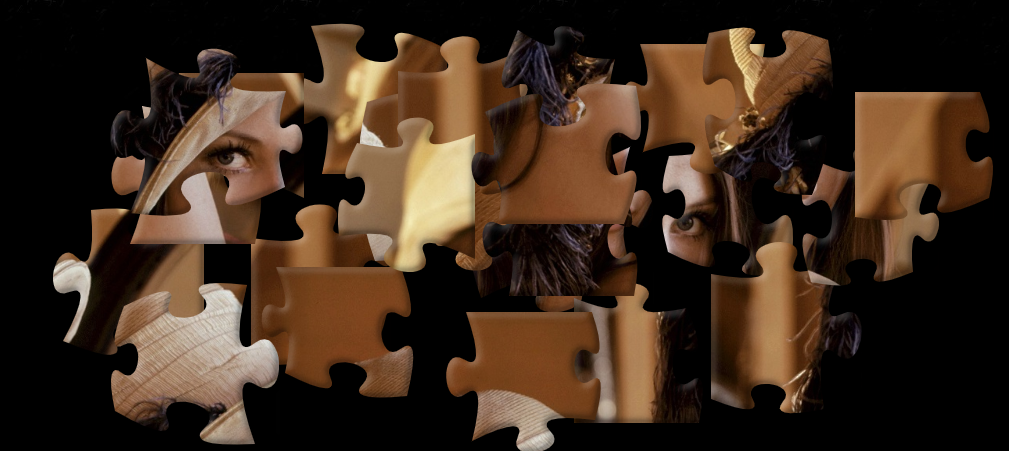
\includegraphics[width=0.70\linewidth]{img/jigex2.png}
    }
    \\
    \subfloat[Teillösung\label{fig-jig-ex-2}]{
        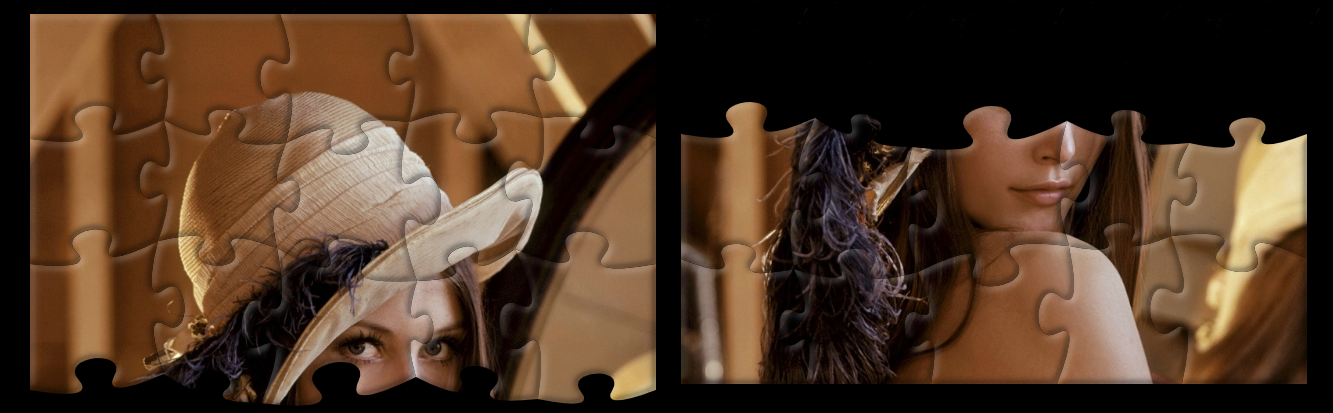
\includegraphics[width=0.60\linewidth,valign=t]{img/jigex3.png}
    }
    \quad
    \subfloat[Lösung\label{fig-jig-ex-3}]{
        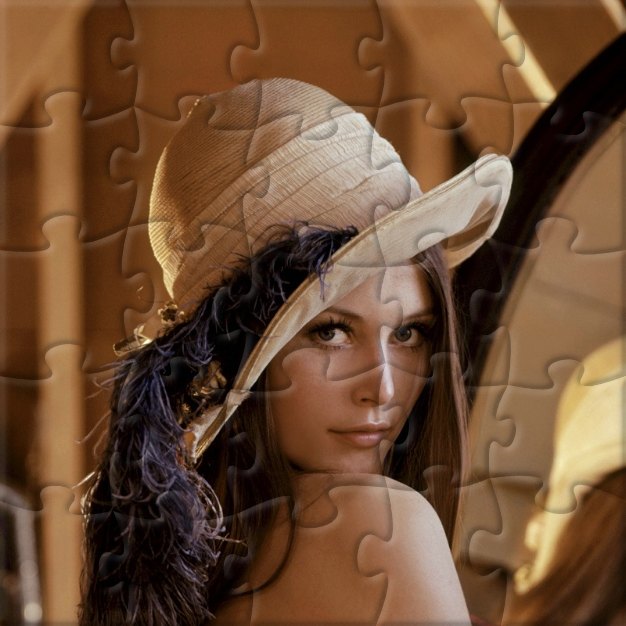
\includegraphics[width=0.30\linewidth,valign=t]{img/jigex1.png}
    }
    \caption{Beispiel eines Jigsaw-Puzzles}
    \label{fig-jig-ex}
\end{figure}
Normalerweise sind die Puzzlestücke dabei speziell geformt (oftmals ähnlich wie in Abb. \ref{fig-jig-ex}). Dies schränkt die Möglichkeiten der gültigen Zusammensetzungen des Puzzles stark ein, besonders da die Möglichkeit besteht zwischen Rahmenstücken und inneren Puzzlestücken zu unterscheiden (Stücke am Rand des Bildes haben mindestens eine glatte Kante). Dadurch entsteht ein Problem, welches sich teilweise nur durch die äußere Form der Puzzlestücke und deren Kompatibilität untereinander lösen lässt. Es gibt sogar Puzzle bei denen diese Information hinreichend ist um das Puzzle vollständig zu lösen (die Stücke selber weisen dann keine weiteren optischen Merkmale auf und sind meist einfarbig).

Mit der Motivation später Schiebepuzzle lösen zu können, muss das Problem auf rechteckige Puzzlestücke verallgemeinert werden. Damit kann weder gesagt werden, ob ein Puzzlestück ein Rahmenstück ist oder sich im inneren des Puzzles befinden muss, noch können Aussagen über die Kompatibilität zweier Puzzlestücke gemacht werden, ohne dabei die Bilder der Puzzlestücke zu analysieren.

Eine noch speziellere Variante von rechteckigen Jigsaw-Puzzles schränkt die Puzzlestücke auf eine quadratische Größe ein. Bei diesen Square Jigsaw Puzzles werden in der Literatur nach \cite{gallagher} zwischen drei Typen unterschieden. Alle Typen haben (sofern nicht anders definiert) Informationen über die Dimensionsgrößen ($m$ Zeilen, $n$ Spalten) des Puzzles. Alle Puzzleteile sind quadratisch (mit der gleichen Seitenlänge) und besitzen Farbinformationen (in Form von einem Bild für jedes Stück). Es gibt exakt $N=m\times n$ Puzzlestücke, womit das Puzzle also keine Lücken oder überschüssige Teile haben wird.

Bei dem Type 1 Square Jigsaw Puzzle ist die Position der Puzzlestücke unbekannt, deren Orientierung jedoch fest und bekannt. Alle möglichen Puzzlestellungen sind dann eine Permutation der vorhandenen Puzzlestücke. Davon gibt es $N!$ verschiedene. Außerdem lassen sich somit zwei Puzzleteile $(x_i,x_j)$ auf vier verschiedene Arten zusammensetzen ($x_i$ kann links, rechts, oben oder unten von $x_j$ platziert werden). Jede Seite von $x_i$ hat nur eine Seite von $x_j$ als möglichen Partner. Das Type 1 Puzzle ist der am meisten untersuchteste Typ von den dreien und hat den Namen \textit{jig swap}\cite{loop} bekommen.

Das Type 2 Puzzle lässt eine unbekannte Orientierung der Puzzleteile zu. Somit lassen die Puzzleteile sich nicht nur anordnen, sondern auch rotieren. Die Anzahl der möglichen Anordnungen des Puzzles vervielfacht sich somit um einen Faktor von $4^N$ auf insgesamt $4^N\cdot N!$. Zwei Puzzlestücke $(x_i,x_j)$ lassen sich nun auf $16$ verschiedene Arten anordnen, da jede Seite von $x_i$ mit jeder Seite von $x_j$ kombiniert werden kann.

Beim Type 3 Puzzle ist die Orientierung zwar unbekannt, die Positionen der Puzzleteile sind jedoch fest und bekannt. Da die Anordnung fest ist und jedes Puzzlestück sich rotieren lässt, hat dieses Puzzle mit $4^N$ möglichen Anordnung die geringste Komplexität. Zwei Puzzlestücke $(x_i,x_j)$ lassen sich auch hier auf $16$ verschiedene Arten kombinieren. Der Unterschied dabei zu Type 1 und Type 2 Puzzles ist jedoch, dass nur die Kompatibilität zwischen Seiten von bereits benachbarten Teilen analysiert werden muss (da die Anordnung fest ist). Bei Type 1 und Type 2 Puzzles kommen für ein Teil $x_i$ alle anderen Teile $x_j,j\neq i$ als mögliche Nachbarn in Frage.

Die Anzahl der möglichen Kombinationen die es gibt, wenn man zwei Seiten von zwei Puzzlestücken vergleichen möchte, ist bereits eine gute untere Schranke für die Laufzeit- und Speicherkomplexität von Algorithmen, welche die Kompatibilität aller Puzzlestücke (in allen möglichen Anordnungen) braucht, um Entscheidungen treffen zu können (um beispielsweise zunächst die Puzzlesteile zu kombinieren, welche von allen die höchste Kompatibilität aufweisen).

Type 1 Puzzle müssen alle Puzzlestücke mit allen anderen Puzzlestücken vergleichen. Da die Kompatibilität zwischen zwei Stücken symmetrisch ist und es $4$ Möglichkeiten gibt die zwei Stücke in einem Type 1 Puzzle anzuordnen ergeben sich somit $$4\binom{N}{2}=2N(N-1)\in\Theta(N^2)$$ Kompatibilitäten die berechnet werden müssen.

Bei Type 2 Puzzle ändert sich lediglich der konstante Faktor vor dem Binomialkoeffizienten von $4$ auf $16$, womit sich auch die Anzahl der berechneten Metriken vervierfach und somit auf $8N(N-1)$ wächst, was weiterhin $\Theta(N^2)$ ist.

Im Gegensatz dazu werden bei Type 3 Puzzles lediglich die Kompatibilitäten zu den benachbarten Puzzlestücken berechnet. Durch die mögliche Rotation der beiden Stücke ergeben sich (wie bei Type 2) $16$ Möglichkeiten pro Paar. Jedes Paar entspricht einer (inneren) Kante im Puzzle (vgl. Abb. \ref{fig-type3}). Die Anzahl der vertikalen Kanten (in der Abbildung rot gekennzeichnet) entspricht $m(n-1)$, die Anzahl der horizontalen Kanten (in der Abbildung grün gefärbt) entspricht dann der Symmetrie nach $n(m-1)$. Damit ergeben sich insgesamt
\begin{align*}
    &16[m(n-1)+n(m-1)]\\
    =&16[2mn-m-n]\\
    =&16(2N-m-n)\in\Theta(N)
\end{align*}
mögliche Kompatibilität, die berechnet werden müssen.
\begin{figure}[H]
    \centering
    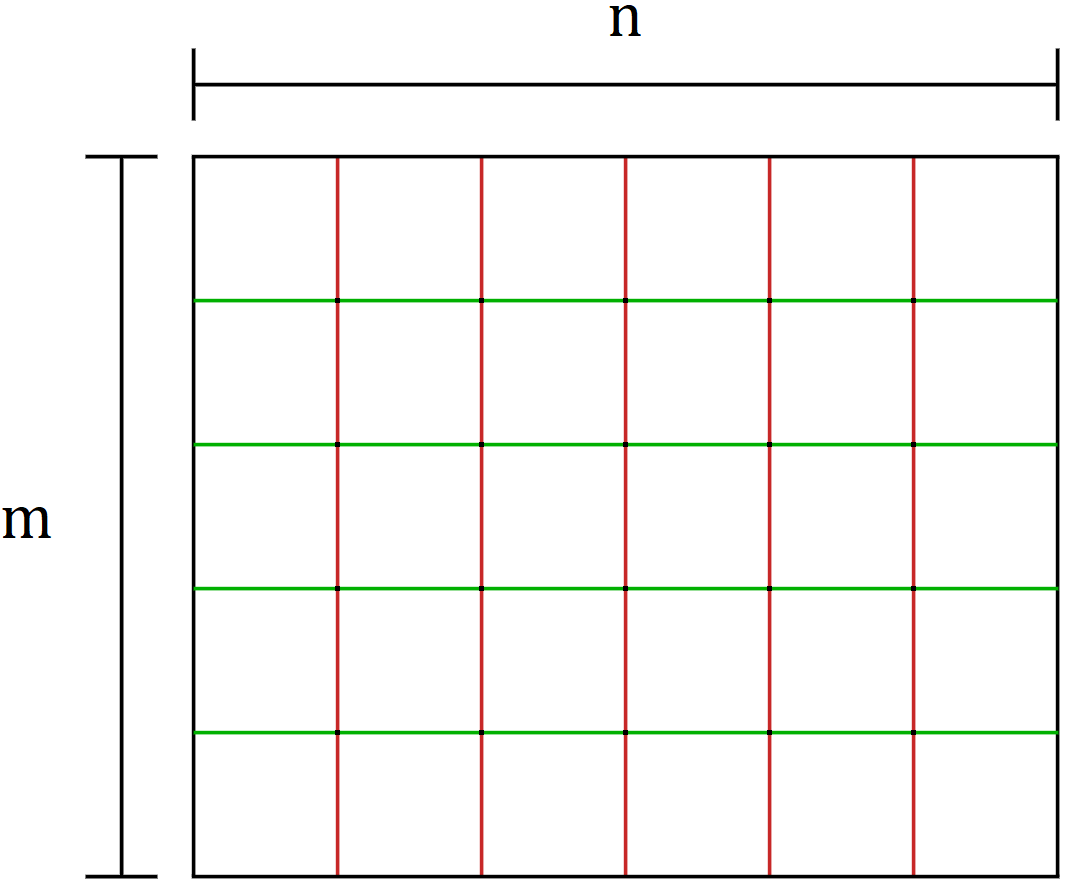
\includegraphics[width=0.60\linewidth]{img/type3.png}
    \caption{Anzahl der Kanten bei einem Type 3 Puzzle}
    \label{fig-type3}
\end{figure}
Es ist zu beachten, dass $N$ bereits quadratisch wächst (bei einem Puzzle mit quadratischen Dimensionen $m=n$). Bei einem $n\times n$ Puzzle ist der Aufwand eines Type 3 Puzzles somit mindestens quadratisch von $n$ abhängig. Bei Type 1 und Type 2 Puzzles wächst dies noch schneller: $\Theta(N^2)=\Theta(n^4)$.

Außerdem sei noch erwähnt, dass mögliche Lösungen beim Type 2 Puzzle aufgrund der erlaubten Rotation (und der Tatsache, dass die Position der Stücke nicht fixiert ist) nicht unbedingt eindeutig sind. Selbst wenn ein Algorithmus es schafft das Bild so zu rekonstruieren, dass jede Seite eines Puzzlestückes den richtigen Partner hat, kann es sein, dass das Gesamtbild jedoch rotiert ist.

Im weiteren Verlauf dieser Arbeit werden hauptsächlich Type 1 Puzzles betrachtet, da Schiebepuzzle sowieso keine Rotation zulassen. Abbildung \ref{fig-jigswap} zeigt ein $8\times 8$ Type 1 Puzzle.
\begin{figure}[H]
    \centering
    \subfloat[Permutiertes Puzzle\label{fig-jigswap-1}]{
      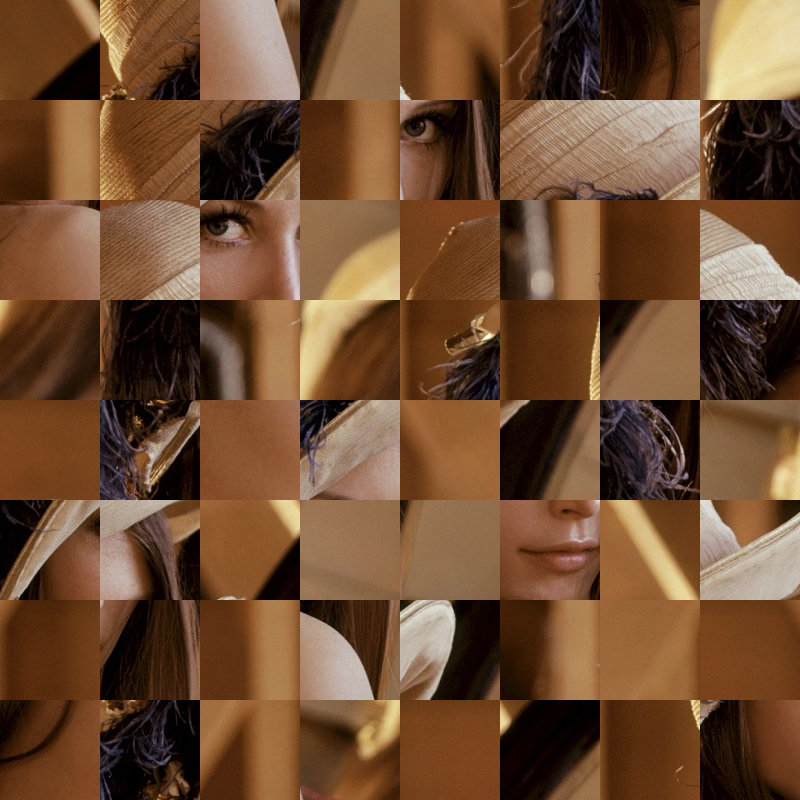
\includegraphics[width=0.30\linewidth]{img/jigswap2.png}
    }
    \quad\quad\quad\quad
    \subfloat[Gelöstes Puzzle\label{fig-jigswap-2}]{
      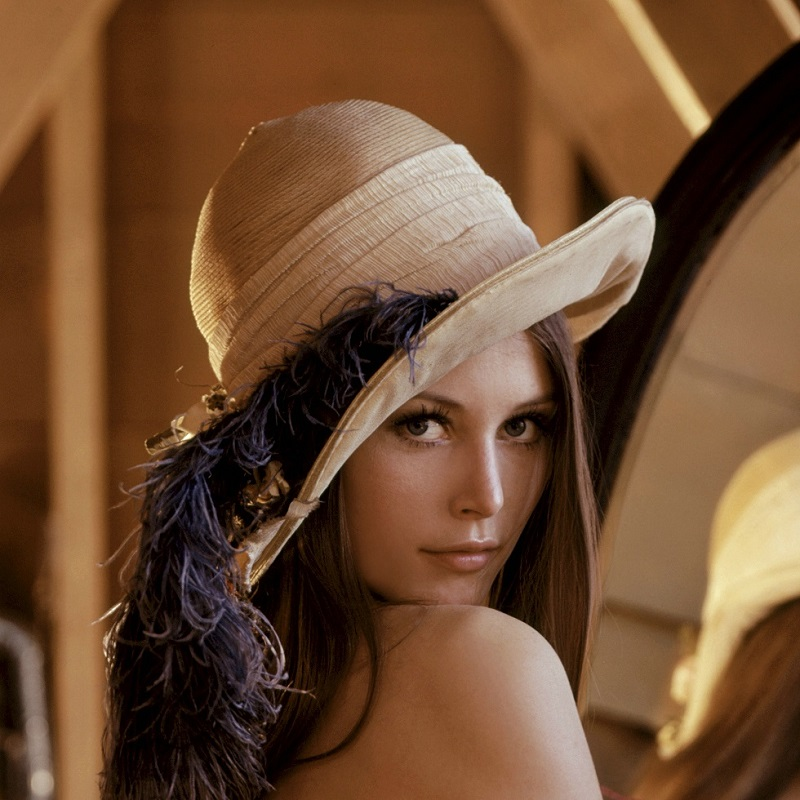
\includegraphics[width=0.30\linewidth]{img/jigswap1.png}
    }
    \caption{Beispiel eines Type 1 Puzzles}
    \label{fig-jigswap}
\end{figure}
Zur Rekonstruktion des Bildes werden Kompatibilitätsmetriken betrachtet, welche später als Information vom eigentlichen Algorithmus verwendet werden, um Entscheidungen zu treffen, welche Puzzlestücke miteinander kombiniert werden sollen und welche nicht.

Genau genommen werden im Folgenden eher Metriken (Distanzfunktionen) betrachtet, die genau das Gegenteil von der Kompatibilität zweier Puzzlestücke darstellen. Den Begriff der Kompatibilität wurde jedoch in \cite{pomeranz} eingeführt und wird seitdem in weiterer Literatur verwendet.
\section{$(L_p)^q$ Norm}\label{section-norm}
Um Aussagen über die Kompatibilität bzw. die Unähnlichkeit (mit Hilfe einer Distanzfunktion) zweier Puzzlestücke zu machen, muss zunächst geklärt werden, wie die Distanz zweier Pixel beschrieben werden kann. Welche Pixel wirklich miteinander verglichen werden beim Vergleich zweier Puzzlestücke ist schließlich erst dann relevant, wenn Möglichkeiten bestehen, die Unähnlichkeit von zwei Pixeln anzugeben.

Da weiterhin Farbbilder aus dem (OpenCV übglichen) BGR-Raum betrachtet werden und somit jeder Pixel drei Channel (mit je 8 Bit) hat, lässt sich ein Pixel als einen Vektor aus dem Raum $[0,256)^3$ auffassen. Damit lässt sich eine Norm $\|\cdot\|:[0,256)^3\rightarrow[0,\infty)$ definieren. Mit einer Norm lässt sich aber mit $d(\vec{u},\vec{v})\coloneqq\|\vec{u}-\vec{v}\|$ eine Metrik einführen.

Die aus der Mathematik bekannte $L_p$ Norm mit $$L_p(\vec{v})=\|\vec{v}\|_p\coloneqq\sqrt[p]{\sum_{i=1}^{n}|v_i|^p},p\in\mathbb{R}^{\geq1}$$ liegt dabei am nächsten. Besonders die $L_2$ Norm (euklidische Norm) oder die $L_1$ Norm (Taxicab Norm oder Manhatten Norm) würden in Frage kommen. In \cite{pomeranz} wurde jedoch für Jigsaw Puzzles mit der $(L_p)^q$ Norm eine weitere (allgemeinere) Norm eigeführt. Die $(L_p)^q$ Norm berechnet sich zu $$(L_p)^q[\vec{v}]=\|\vec{v}\|_p^q\coloneqq \sqrt[\leftroot{-2}\uproot{5}\frac{p}{q}]{\sum_{i=1}^{n}|v_i|^p}$$.

Die $(L_p)^q$ Norm ist damit die mit $q$ potenzierte $L_p$ Norm: $(L_p)^q[\vec{v}]\coloneqq(L_p[\vec{v}])^q$. Auch in \cite{pomeranz} (empirisch) gezeigt wurde, dass besonders $p=\frac{3}{10}$ und $q=\frac{1}{16}$ gute Ergebnisse liefern.
\section{Dissimilarity-Based Compatibility (DBC)} \label{section-dbc}
Die erste Metrik beschrieben in \cite{pomeranz} ist die Dissimilarity-Based Compatibility (DBC). Diese summiert die Distanzen zweier Puzzlestücke entlang einer Kante auf. Da es für Type 1 Puzzle vier verschiedene Möglichkeiten gibt, zwei Stücke $x_i$ und $x_j$ anzuordnen, wird zunächt eine numerische Konstante $r\in\{0,1,2,3\}$ definiert, die diesen Zusammenhang darstellt.
\begin{table}[H]
    \centering
    \begin{tabular}{c|c|c|c}
        $r=0$ & $r=1$ & $r=2$ & $r=3$\\
        \hline
        \begin{tikzpicture}
            \draw (0,0) rectangle (1,1) node[midway] {$x_i$};
            \draw (1,0) rectangle (2,1) node[midway] {$x_j$};
        \end{tikzpicture}&
        \begin{tikzpicture}
            \draw (0,0) rectangle (1,1) node[midway] {$x_j$};
            \draw (0,1) rectangle (1,2) node[midway] {$x_i$};
        \end{tikzpicture}&
        \begin{tikzpicture}
            \draw (0,0) rectangle (1,1) node[midway] {$x_j$};
            \draw (1,0) rectangle (2,1) node[midway] {$x_i$};
        \end{tikzpicture}&
        \begin{tikzpicture}
            \draw (0,0) rectangle (1,1) node[midway] {$x_i$};
            \draw (0,1) rectangle (1,2) node[midway] {$x_j$};
        \end{tikzpicture}
    \end{tabular}
    \caption{Räumlicher Zusammenhang zweier Puzzlestücke}
    \label{tbl-spatial-relation}
\end{table}
Die DBC entlang einer Kante, die beim Zusammensetzen zweier Puzzlestücke entsteht, wird dann mit $D(x_i,x_j,r)$ bezeichnet. Da diese Metrik symmetrisch ist gilt außerdem $D(x_i,x_j,r)=D(x_j,x_i,r^\prime)$. Wobei $r^\prime$ die inverse Relation der beiden Puzzlestücke darstellt und sich zu $$r^\prime=(r+2)\bmod4$$ berechnet.

Als Referenzstellung der beiden Puzzleteile wird im weiteren Verlauf $r=0$ verwendet ($x_i$ befindet sich also links von $x_j$). Andere Stellungen lassen sich entweder ähnlich berechnen (lediglich durch das Vertauschen der Dimensionen oder durch das Vertauschen von $i$ und $j$) oder sogar gleich berechnen, sofern die beiden Puzzlestücke zuvor entsprechend rotiert wurden.

Diese DBC zweier Puzzlestücke $x_i(x,y)$ und $x_j(x,y)$ mit Höhe $h$ und Breite $w$ und basierend auf einer Norm $\|\cdot\|$ berechnet sich dann zu:
\begin{align} \label{eq-dbc}
    D(x_i,x_j,0)=\sum_{k=0}^{h-1}\|x_i(w-1,k)-x_j(0,k)\|
\end{align}
.

Da diese Distanz bei rechteckigen Puzzlestücken die kürzeren Seiten generell bevorzugt (die Summanden sind stets positiv, womit selbst gute Kanten bei vielen Summanden große Werte liefern), kann diese Distanz noch durch die Anzahl der Summanden bzw. die Länge der Seite $K$ (bei $r=0$ beispielsweise die Höhe der Puzzlestücke) dividiert werden: $$\bar{D}(x_i,x_j,r)=\frac{1}{K}\cdot D(x_i,x_j,r)$$.

Um diese Distanz gegebenenfalls noch auf das Intervall $[0,1]$ zu normalisieren, lässt sich die durchschnittliche Distanz (pro Summand) durch die maximale Distanz $d_{max}$ zwischen zwei Pixel dividieren. Diese maximale Distanz hängt von der gewählten Norm ab. Bei der euklidischen Norm ist dies beispielsweise $d_{max}=\sqrt{255^2+255^2+255^2}=\sqrt{3\cdot255^2}=\sqrt{3}\cdot255$.

Damit lässt sich nun die Kompatibilität zweier Puzzlestücke als die Gegenwahrscheinlichkeit dieser relativen Distanz definieren:$$C(x_i,x_j,r)\coloneqq 1-\frac{\bar{D}(x_i,x_j,r)}{d_{max}}$$.

Die DBC bietet eine simple Möglichkeit die Kompatibilität (oder Distanz) zwischen zwei Puzzlestücken zu berechnen. Die Berechnung einer solchen Distanz bezüglich einer Kante ist linear in der Länge dieser Kante $\Theta(K)$ (Höhe oder Breite der Puzzlestücke). Ein Nachteil ist, dass lediglich die äußersten Pixel eines Puzzlestückes betrachtet werden. Dadurch werden Farbübergänge, die zwar im Gesamtbild Sinn ergeben, an den Kanten als harsch angesehen, da diese dort für große Distanzen sorgen.
\section{Prediction-Based Compatibility (PBC)}\label{section-pbc}
Um neben den Randpixeln auch noch die Informationen von deren (inneren) benachbarten Pixeln nutzen zu können, wird bei der Prediction-Based Compatibility (PBC) das Bild eines Puzzlestückes um einen Pixel in jede Richtung erweitert. Diese approximierten Pixel einer Seite werden dann anstatt den eigentlichen Pixeln dieser Seite (wie es bei der DBC der Fall ist) in der Distanzberechnung verwendet. Es wird also die Distanz zwischen einem approximierten Pixel in einem Puzzlestück und einem echten Pixel in einem anderen Puzzlestück ermittelt.

Zur Approximierung der Farbwerte lässt sich ein Bild $I$ mit der Breite $w$ und der Höhe $h$ im BGR-Farbraum wieder als vektorwertige Funktion $\vec{I}(\vec{x}):[0,w)\times[0,h)\rightarrow[0,256)^3$ betrachten. Es wird eine lineare Approximierung nach Taylor gewählt. Um eine Entwicklungsstelle $\vec{x}_0$ gilt dann $$\vec{I}(\vec{x})\approx\vec{I}(\vec{x}_0)+J_I(\vec{x}_0)\cdot(\vec{x}-\vec{x_0})$$. Wobei mit $J_I(\vec{x}_0)$ die Jacobi-Matrix (ausgewertet an der Entwicklungsstelle $\vec{x}_0$) gemeint ist. Die Jacobi-Matrix fasst alle partiellen Ableitungen der Funktion zusammen (die Komponenten von $I$ werden entsprechend der Farbchannel als $b$, $g$ und $r$ bezeichnet): $$J_I=\begin{bmatrix}\frac{\partial b}{\partial x}&\frac{\partial b}{\partial y}\\\frac{\partial g}{\partial x}&\frac{\partial g}{\partial y}\\\frac{\partial r}{\partial x}&\frac{\partial r}{\partial y}\end{bmatrix}$$.

Um die einzelnen Ableitungen numerisch zu bestimmen, werden finite Differenzen verwendet. Dabei wird unterschieden zwischen dem Forward-Differenzenquotienten $\Delta_F[f](x)$, Backward-Differenzenquotienten $\Delta_B[f](x)$ und Central-Differenzenquotienten $\Delta_C[f](x)$.
\begin{align*}
    \Delta_F[f](x) &= \frac{f(x+h)-f(x)}{h}\\
    \Delta_B[f](x) &= \frac{f(x)-f(x-h)}{h}\\
    \Delta_C[f](x) &= \frac{\Delta_F[f](x)+\Delta_B[f](x)}{2}\\
                   &= \frac{f(x+h)-f(x-h)}{2h}
\end{align*}
Der Central-Differenzenquotient ist damit also das arithmetische Mittel vom Forward-Differenzenquotienten und vom Backward-Differenzenquotienten. Da die Ableitung einer Funktion $f$ an einer Stelle $x$ gerade der Grenzwert dieser Quotienten darstellt, für die $h\rightarrow0$, werden zur numerischen Berechnung kleine $h\neq0$ gewählt. Die Koordinaten $(x,y)$ eines Bildes können jedoch nur diskrete Werte annehmen, womit das kleinstmögliche $h$ somit $h=1$ ist. Das Aufstellen der Differenzenquotienten für vektorwertige Funktionen lässt sich analog zum skalaren Beispiel konstruieren (wobei die Funktionsdifferenz im Zähler dann eine Vektordifferenz ist, anders gesagt wird der Differenzenquotient für jede Komponente gebildet). Für Funktionen, die von mehreren Variablen abhängig sind, entsprechen die Differenzenquotienten dann einer Approximierung der partiellen Ableitungen, wobei lediglich der Parameter variiert wird, nach dem abgeleitet werden soll. Die restlichen Parameter werden konstant gehalten.

Als Beispiel lässt sich somit ein Bild an den Rändern erweitern, indem der nächstgelegene Pixel als Entwicklungsstelle für die lineare Approximierung genommen wird. In Abbildung \ref{fig-pred} wird gezeigt, wie ein Bild sowohl nach oben als auch nach rechts um jeweils einen Pixel erweitert wird.

Ein Pixel am (erweiterten) rechten Rand (in der Zeile $y$) des Bildes hat die Koordinaten $(w,y)$. Als Entwicklungsstelle wird der links benachbarte Pixel mit den Koordinaten $(w-1,y)$ gewählt. Der Farbwert des neuen (erweiterten) Pixels lässt sich dann mit
\begin{align} \label{eq2}
    \vec{I}(w,y) &= \vec{I}(w-1,y) + \begin{bmatrix}
        \frac{\partial \vec{I}}{\partial x} &
        \frac{\partial \vec{I}}{\partial y}
    \end{bmatrix}
    \biggr \rvert_{(x,y)=(w-1,y)} \cdot
    \left( \begin{bmatrix}
        w \\
        y
    \end{bmatrix} - \begin{bmatrix}
        w-1 \\
        y
    \end{bmatrix} \right),&\forall y:0\leq y<h \nonumber \\
    &= \vec{I}(w-1,y) + \begin{bmatrix}
        \vec{I}_x(w-1,y) & \vec{I}_y(w-1,y)
    \end{bmatrix} \cdot \begin{bmatrix}
        1 \\
        0
    \end{bmatrix} \nonumber \\
    &= \vec{I}(w-1,y) + \vec{I}_x(w-1,y)
\end{align}
approximieren.

Bei der numerischen Approximierung der partiellen Ableitung von $\vec{I}$ entlang der $x$-Achse kommt ausschließlich der Backward-Differenzenquotient in Frage. Dies liegt daran, dass die Pixel mit einer $x$-Koordinate von $w-1$ sich in der letzten Spalte des Bildes befinden und somit entlang der $x$-Achse keinen rechts benachbarten Pixel haben. Damit ergibt sich:
\begin{align} \label{eq3}
    \vec{I}_x(w-1,y) &= \Delta_B\left[\vec{I}\right](w-1,y) \nonumber \\
    &= \frac{\vec{I}(w-1,y)-\vec{I}(w-1-h,y)}{h} \nonumber \\
\shortintertext{Mit $h=1$ folgt}
    \vec{I}_x(w-1,y) &= \vec{I}(w-1,y)-\vec{I}(w-2,y)
\end{align}
Insgesamt ergibt sich mit \ref{eq2} und \ref{eq3} die vollständige Formel zu Berechnung des erweiterten Randes vom Bild.
\begin{align} \label{eq4}
    \vec{I}(w,y)=2\vec{I}(w-1,y)-\vec{I}(w-2,y)
\end{align}
Die Formulierung einer solchen Approximierung für Pixel an anderen Seiten des Bildes lässt sich ähnlich angeben. Lediglich bei der Approximierung der Pixel in einer (neuen) Ecke des Bildes müssen beide partiellen Ableitungen approximiert werden (als Entwicklungsstelle wird die alte Ecke des Bildes genommen, womit sowohl ein Schritt entlang der x-Achse, also auch einen Schritt entlang der y-Achse gegangen wird).

Außerdem ist noch zu beachten, dass mit der reinen Berechnung nach \ref{eq4} noch nicht sichergestellt ist, dass die Channel des neuen Pixels sich auch wieder in dem Wertebereich $[0,256)$ befinden. Es gilt also zu beachten, dass die Berechnung keine modulare Arithmetik verwenden sollte (dazu sollte die Berechnung in einem größeren Vorzeichen behafteten Datentyp stattfinden). Um die Werte danach wieder auf das Intervall $[0,256)$ zu bringen, sollte dann unbedingt der in \ref{section-sat} angesprochene \texttt{cv::saturate\_cast<>()} verwendet werden.

Der folgende Ausschnitt an Quelltext zeigt, wie die Berechnung nach \ref{eq4} mit einem Quellbild \texttt{src} und einem Zielbild \texttt{dst} in OpenCV umgesetzt werden kann.
\begin{lstlisting}[caption=Lineare Approximierung (nach Taylor) von Pixel am rechten Bildrand, label=lst-pred-sat]
for (size_t row = 0; row < src.rows; row++)
{
    for (size_t ch = 0; ch < 3; ch++)
    {
        dst.at<cv::Vec3b>(row, src.cols)[ch] =
            cv::saturate_cast<cv::uchar>(
                  2 * dst.at<cv::Vec3b>(row, src.cols - 1)[ch]
                -     dst.at<cv::Vec3b>(row, src.cols - 2)[ch]
            )
        ;
    }
}
\end{lstlisting}
Um den \texttt{cv::saturate\_cast<>()} geeignet anwenden zu können, werden die Pixel im Quelltext Channel für Channel durchgegangen (Schleife in Zeile 3). Außerdem wird mit der Multiplikation der numerischen Konstante $2$ in Zeile 7 die komplette Berechnung implizit zu einer Berechnung mit Integer Werten. Wäre dies hier nicht der Fall, würde auch die Saturierung des berechneten Wertes nichts daran ändern, dass bereits bei der Berechnung selber gegebenenfalls Over- oder Underflows aufgetreten sind.

Abbildung \ref{fig-pred} zeigt neben dem Ausgangsbild und der oberen rechten Ecke dieses Bildes, zwei Varianten zur Berechnung der Approximierung.

In \ref{fig-pred-nosat} wurde der Saturate-Cast weggelassen, wodurch der (zunächst richtig) berechnete Wert bei der Zuweisung an einen kleineren Datentypen die Informationen in den höheren Bits verliert. Als Ergebnis entstehen einzelne Pixel, die stark vom eigentlichen Bildverlauf abweichen. Suggerieren zwei benachbarte Pixel etwa einen immer dunkler werdeden Farbverlauf, so kann es vorkommen, dass der approximierte Pixel als so dunkel angenommen wird, dass die Werte der Channel bei der Berechnung negativ werden. Diese Annahme ist nicht falsch. Ein impliziter Cast zu einem \texttt{uchar} bewirkt dann jedoch, dass die Channel sehr große Werte annehmen. Das bereits beschriebene Clamping vom Saturate-Cast verhindert dies, sodass ein überaus dunkler Pixel in jedem Channel gegebenenfalls auf den dunkelsten Wert (welcher $0$ entspricht) gesetzt wird. Die gleiche Berechnung mit einem Saturate-Cast liefert, wie in \ref{fig-pred-sat} zu sehen ist, eine zum Farbverlauf passende und somit realistisch aussehende Approximierung der neuen Randpixel.
\begin{figure}[H]
    \centering
    \subfloat[Originalbild\label{fig-pred-orig}]{
      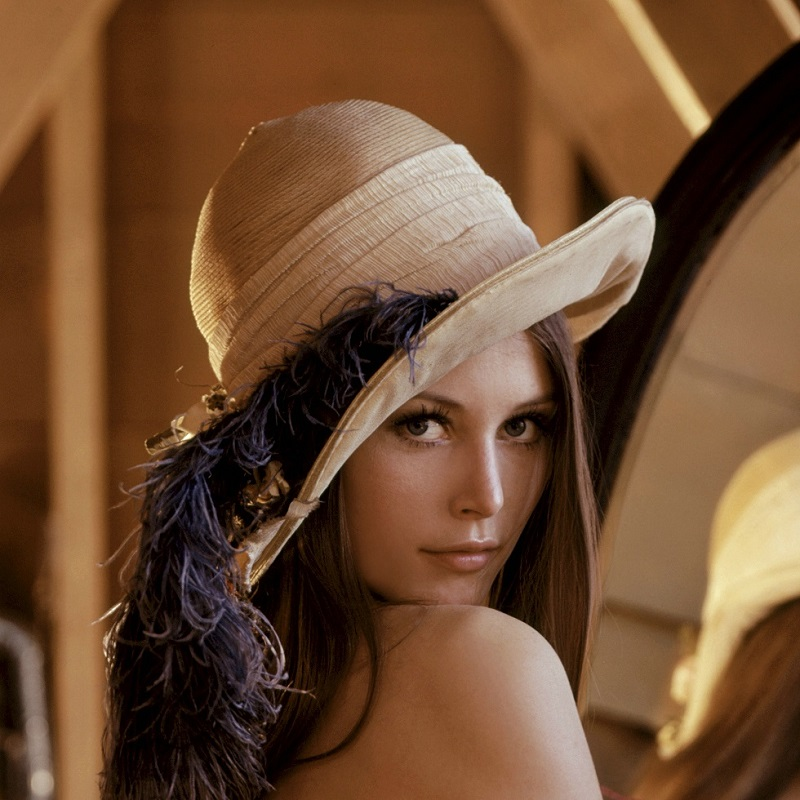
\includegraphics[width=0.40\linewidth,valign=t]{img/linear_orig.png}
    }
    \quad\quad
    \subfloat[Obere rechte Ecke im Originalbild\label{fig-pred-orig2}]{
      
\includegraphics[width=0.20\linewidth,valign=t]{img/linear_orig2.png}
    }
    \\
    \subfloat[Berechnung ohne Saturierung\label{fig-pred-nosat}]{
        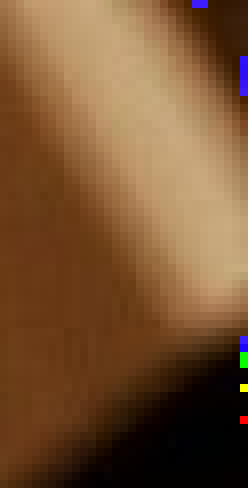
\includegraphics[width=0.20\linewidth]{img/linear_nosat.png}
    }
    \quad\quad\quad\quad\quad\quad\quad\quad
    \subfloat[Berechnung mit Saturierung\label{fig-pred-sat}]{
        
\includegraphics[width=0.20\linewidth]{img/linear_sat.png}
    }
    \caption{Lineare Approximierung der Pixel am rechten und am oberen Bildrand}
    \label{fig-pred}
\end{figure}
Um diese Art der Approximierung nun zu nutzen um die Kompatibilität zweier Puzzlestücke herauszufinden, wird ähnlich wie in \ref{section-dbc} vorgegangen. Als Referenzstellung wird wieder $r=0$ gewählt, womit sich ein Puzzlestück $x_i$ links von einem anderen Puzzlestück $x_j$ befindet. Dabei wird die Berechnung diesmal jedoch in zwei Teile eingeteilt. Es wird zunächst die Distanz betrachtet, die entsteht wenn man die rechte Seite von $x_i$ approximiert und mit den (echten) Pixeln der linkten Seite von $x_j$ vergleicht. Diese Distanz $D_L$ berechnet sich dann analog zu der DBC in \ref{eq-dbc}. Der einzige Unterschied besteht darin, dass die approximierte Spalte an Pixeln von $x_i$ genommen wird. In der Formel aus \ref{eq-dbc} wird also das $x_i(w-1,k)$ zu einem $x_i(w,k)$ geändert, was für die Pixel in der (nicht existierenden, aber approximierten) Spalte von $x_i$ steht. Dann ergibt sich:
\begin{align}\label{eq-DL}
    D_L(x_i,x_j,0)&=\sum_{k=0}^{h-1}\|x_i(w,k)-x_j(0,k)\| \nonumber \\
\shortintertext{Entsprechend der Approximierung in \ref{eq4} lässt sich $x_i(w,k)$ aber als die Linearkombination zweier echten Pixel von $x_i$ berechnen}
    D_L(x_i,x_j,0)&=\sum_{k=0}^{h-1}\|2x_i(w-1,k)-x_i(w-2,k)-x_j(0,k)\|
\end{align}
Um weiterhin garantieren zu können, dass die Distanz zwischen zwei Puzzlestücken symmetrisch ist, wird die Gesamtdistanz zweier Puzzlestücke als die Summe beider Distanzen der Approximierungen gebildet. Dazu wird nun $D_R(x_i,x_j,0)$ ähnlich wie in \ref{eq-DL} berechnet.
\begin{align}\label{eq-DR}
    D_R(x_i,x_j,0)&=\sum_{k=0}^{h-1}\|x_i(w-1,k)-2x_j(0,k)+x_j(1,k)\|
\end{align}
Wurden beide Seiten berechnet, so lässt sich die gesamte Distanz zu $D(x_i,x_j,r)=D_L(x_i,x_j,r)+D_R(x_i,x_j,r)$ berechnen. Damit ist sichergestellt, dass weiterhin der Symmetrie nach $D(x_i,x_j,r)=D\left(x_i,x_j,\left(r+2\right)\bmod4\right)$ gilt.

Da ähnlich wie bei der DBC in \ref{section-dbc} die Distanzen entlang einer Kante aufsummiert werden, ist die Berechnung einer Distanz linear in der Länge dieser Kante. Bei der PBC kommen entsprechend noch zusätzliche Berechnung zur Approximierung der Pixel dazu. Um die Anzahl der konstanten Schritte möglichst minimal zu halten (im Austausch von zusätzlichem Speicherplatz), lassen sich die approximierten Seiten eines Puzzlestückes nur einmal initial berechnen und dann zwischenspeichern. Damit müssen für jedes der $N$ Puzzlestücke zwei horizontale Kanten der Breite $w$ (oben und unten) und zwei vertikale Kanten der Höhe $h$ (links und rechts) abgespeichert werden. Insgesamt müssen damit $2N(w+h)$ Pixel berechnet und abgespeichert werden (alle jeweils mit drei Channel).
\section{Dynamic Time Warping (DTW)}\label{section-dtw}
Eine weitere Methode zur Berechnung der Gesamtdistanz zwischen zwei Puzzlestücken wurde in \cite{hungarian} beschrieben. Intuitiv betrachtet lässt sich vermuten, dass der Vergleich zweier Pixel sich nicht nur auf unmittelbar benachbarte Pixel entlang einer Achse (beispielsweise linke und rechte Nachbarn) beschränken sollte.

Abbildung \ref{fig-dtw-ex} zeigt als Beispiel zwei $8\times1$ Bildränder: $R$ (etwa der rechte Bildrand eines Puzzlestückes $x_i$) und $S$ (der linke Rand eines anderen Puzzlestückes $x_j$). Diese sollen beispielsweise nach \ref{section-dbc} mit der DBC verglichen werden. Wird als Norm die $L_1$ Norm gewählt (Summe der absoluten Differenzen oder auch Manhatten oder Taxicab-Norm), ergibt sich nach dem aufsummieren dieser $8$ Distanzen eine Gesamtdistanz von $2246$.
\begin{figure}[H]
    \centering
    \subfloat[$R$\label{fig-dtw-ex-a}]{
      
\includegraphics[width=0.06\linewidth]{img/dtw_ex_a.png}
    }
    \quad\quad\quad\quad
    \subfloat[$S$\label{fig-dtw-ex-b}]{
      
\includegraphics[width=0.06\linewidth]{img/dtw_ex_b.png}
    }
    \caption{Direkte Zuordnung der Pixel}
    \label{fig-dtw-ex}
\end{figure}
Die Farben in Beispiel \ref{fig-dtw-ex} suggerieren bereits, dass eine andere Zuordnung, welche nicht nur ausschließlich direkt benachbarte Pixel vergleicht, eine geringere Distanz ergeben könnte. So würde beispielsweise das Verschieben von $S$ um einen Pixel nach unten dafür sorgen, dass viele ähnliche Pixel (blau mit blau und grün mit grün) verglichen werden könnte.

Ein Algorithmus der dieses Problem behandelt ist der Dynamic Time Warping (DTW) Algorithmus. Ursprünglich wurde der Algorithmus entwickelt, um die best mögliche Zuordnung (die Zuordnung mit der geringsten Distanz bzw. mit der größten Ähnlichkeit) von zwei zeitabhängigen Sequenzen zu bestimmen (die nicht zwingend gleicher Länge sein müssen). Möchte man beispielsweise Aussagen über die Ähnlichkeit zweier Audiosignale machen, in denen zwei verschiedene Personen die gleiche Sequenz von Wörtern vorlesen (ein Anwendungsbeispiel aus dem Bereich der automatische Spracherkennung), so würde ein direkter Vergleich der beiden Signale auf zwei grundlegende Probleme stoßen: Werden ausschließlich die Frequenzen verglichen, die in den Signalen am gleichen Zeitpunkt $t$ auftreten, so müsste vorausgesetzt werden, dass die beiden Signale die gleiche Länge $T$ haben, was aufgrund der unterschiedlichen Sprachgeschwindigkeit von Menschen sehr unwahrscheinlich ist. Und selbst wenn beide Signale eine gleiche Länge aufweisen, so sorgt genau diese Sprachgeschwindigkeit dafür, dass gegebenenfalls ein Signal zeitlich immer leicht verschoben ist. Somit würden zwei ähnliche Signale als komplett verschieden anerkannt werden, weil bei der Zuordnung der Frequenzen nicht beachtet wird, dass gleiche Frequenzen zeitverschoben auftreten können. Abbildung \ref{fig-dtw-vs} zeigt zwei Beispiel Matchings einer zeitabhängigen Sequenz. Eine direkte Zuordnung (euklidisches Matching) sorgt dafür, dass zeitlich verschobene aber ähnliche Frequenzen nicht einander zugeordnet werden können. Der DTW-Algorithmus findet das beste Matching, indem die Sequenzen so \textit{verzerrt} werden, dass diese Zuordnung der ähnlichen Frequenzen möglich wird.
\begin{figure}[H]
    \centering
    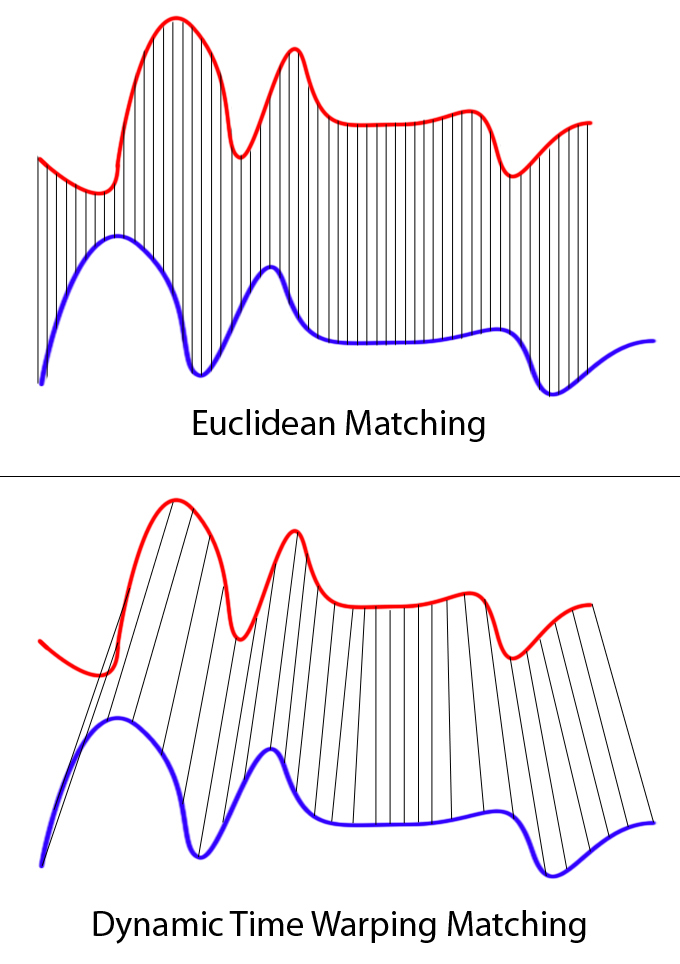
\includegraphics[width=0.60\linewidth]{img/eu_vs_dtw.jpg}
    \caption{Euclidean Matching im Vergleich mit DTW}
    \caption*{Quelle: Wiki Commons: File:Euclidean vs DTW.jpg (\url{https://commons.wikimedia.org/wiki/File:Euclidean_vs_DTW.jpg})}
    \label{fig-dtw-vs}
\end{figure}
Im Gegensatz zu zeitabhängigen Sequenzen (welche ein Beispiel für stetige Sequenzen sind) ist die Zuordnung zwischen zwei Pixelsequenzen diskret, da es nur eine endliche Anzahl an Indizes gibt. Bevor der Algorithmus selber beschrieben werden kann, sollte festgelegt werden, welche Eigenschaften eine Zuordnung aufweisen muss um gültig zu sein (bzw. welche Matchings zulässig sind).

Es werden zwei Sequenzen $R=(r_1,\dots,r_m)$ und $S=(s_1,\dots,s_n)$ betrachtet, mit entsprechenden Längen $|R|=m$ und $S=n$ (im konkreten Fall, wo $R$ und $S$ Seitenränder von Puzzlestücken sind gilt natürlich $m=n$). Auf den Elementen der Sequenz sei eine Metrik bzw. Distanzfuntkion $d(r_i,r_j)$ definiert. Bei den Bildpunkten lässt sich die Matrik mit einer Norm $\|\cdot\|$ nach \ref{section-norm} als $d(r_i,r_j)=\|r_i-r_j\|$ definieren. Gesucht ist die minimale Gesamtdistanz $D$ als Summe einzelner Distanzen durch das Matching jeweils zweier Elemente aus den Sequenzen $D(R,S)=\sum_{i,j}d(r_i,r_j)$. Dieses Matching muss folgende Eigenschaften beachten:
\begin{enumerate}
    \item Jedes Element muss mindestens einen Summanden zur Gesamtdistanz beitragen. Anders gesagt muss jedes Element aus einer Sequenz mit mindestens einem Element aus der anderen Sequenz verbunden werden. Es existieren also keine Elemente, die bei der Berechnung nicht in die Gesamtdistanz mit einfließen.
    \item Ein Matching $(r_i,s_j)$ besagt, dass das Element $r_i$ mit dem Element $s_j$ verbunden wurde (es wird also $d(r_i,s_j)$ aufsummiert). Existiert solch ein Matching $(r_i,s_j)$, dann darf kein Matching $(r_k,s_l)$ existieren mit $(k<i\land l>j)\lor (k>i\land l<j)$. Anschaulich bedeutet dies, dass Zuordnungen sich nicht überkreuzen dürfen (wie auch in Abbildung \ref{fig-dtw-vs} zu sehen ist.
    \item Zusammen implizieren Punkt 1 und 2 damit außerdem, dass beide Anfangs- und Endelemente der beiden Sequenzen stets in Verbindung stehen. Es existieren also mit Sicherheit die Verbindungen $(r_1,s_1)$ und $(r_m,s_n)$. Um dies zu begründen, wird die Verbindung $(r_1,s_1)$ betrachtet (die Begründung für beide Endelemente der Sequenzen geht analog). Nach Punkt 1 muss mindestens ein Matching $(r_1,s_k)$ existieren. Ist $k=1$, so gilt Punkt 3 trivialerweise. Andernfalls kann $k$ nur größer $1$ sein. Jetzt gilt nach Punkt 1 wieder, dass aber auch eine Verbindung $(r_l,s_1)$ existieren muss. Wählt man nun auch ein $l>1$, so existieren gleichzeitig die Verbindungen $(r_1,s_{k>1})$ und $(r_{l>1},s_1)$. Nach Punkt 2 kreuzen die beiden Verbindungen sich dann aber. Es würde also nur ein $l\leq1$ in Frage kommen. Das einzige $l$ was damit in Frage kommt, wäre $l=1$. Auch damit existiert also wieder die Verbindung $(r_1,s_1)$.
\end{enumerate}
Der DTW-Algorithmus arbeitet rekursiv. Dabei werden Teillösungen der Gesamtdistanz $D(R,S)$ betrachtet, die sich auf die Gesamtdistanz zwischen einem Präfix von $R$ und einem Präfix von $S$ beziehen. Diese Zwischenlösungen werden im Folgenden als $D_{i,j}(R,S)$ geschrieben und stellen die Gesamtdistanz zwischen den ersten $i$ Elementen von $R$ und den ersten $j$ Elementen von $S$ dar. Es gilt also $D_{i,j}(R,S)\coloneqq D((r_1,\dots,r_i),(s_1,\dots,s_j))$. Die am Ende gesuchte Gesamtdistanz von allen Elementen von $R$ und allen Elementen von $S$ ist dann $D(R,S)\coloneqq D_{m,n}(R,S)$. Mit dieser Schreibweise lässt sich der Algorithmus dann folgendermaßen rekursiv definieren:
\begin{align}\label{eq-dtw-cases}
    D_{i,j}(R,S)=\begin{cases}
        0&i=0\land j=0\\
        d(r_i,s_j)+\min\begin{cases}
            D_{i-1,j}(R,S)\\
            D_{i,j-1}(R,S)\\
            D_{i-1,j-1}(R,S)
        \end{cases}&1\leq i\leq m\land1\leq j\leq n\\
        \infty&\text{sonst}
    \end{cases}
\end{align}
Der erste Fall ist der Basisfall, wo die Gesamtdistanz von zwei leeren Sequenzen berechnet werden soll. Da somit keine Verbindungen zwischen Elementen entstehen können und somit auch keine Distanzen berechnet werden können, wird definiert dass $D(\varnothing,\varnothing)=0$. Beim dritten Fall der Fallunterscheidung handelt es sich auch um einen Basisfall. Hier ist $i=0\lor j=0$ nicht aber $i=0\land j=0$. Damit soll die Gesamtdistanz von einer nicht leeren Sequenz und einer leeren Sequenz berechnet werden. Da jedoch jedes Element mindestens Teil einer Verbindung sein muss und es keine möglichen Partner für Elemente aus der nicht leeren Sequenz gibt (da die andere Sequenz leer ist), wird die Distanz hier als maximal bzw. $\infty$ definiert. Da der Algorithmus probiert zu minimieren, wird also niemals eine Zuordnung gewählt, die im Laufe des Algorithmus auf solch einen Fall trifft (da offensichtlich nicht alle Elemente einen Partner zugewiesen bekommen haben und das Matching somit nicht gültig ist). Im Rekursionsschritt werden dann die Elemente $r_i$ und $s_j$ verbunden und deren Distanz $d(r_i,s_j)$ berechnet und mit der minimalen Distanz aller Rekursionsfälle addiert. Dabei wird zwischen drei Fällen unterschieden. Da sowohl $r_i$ als auch $s_j$ nun mindestens einen Partner besitzen, lassen sich diese von den jeweiligen Sequenzen ausschließen und es kann mit dem entsprechenden Präfix der Sequenz weitergerechnet werden. Dabei können beide ausgeschlossen werden, womit im weiteren Verlauf keine Verbindung mehr mit $r_i$ oder $s_j$ hergestellt werden kann oder es wird genau einer von beiden ausgeschlossen, wobei der jeweils andere in der nächsten Rekursionstiefe wieder eine (weitere) Verbindung mit dem Vorgänger von dem ausgeschlossenen Element aufbaut. Es sei zu beachten, dass zu keiner Zeit im Algorithmus eine Verbindung mit einem Element aufgebaut werden kann, welches sich außerhalb der beiden Präfixe befindet. Damit ist implizit sichergestellt, dass ein Matching nie zwei Verbindung enthält, welche sich kreuzen.

Da eine rekursive Implementation nach \ref{eq-dtw-cases} gleiche Teilprobleme öfters berechnet, ergibt sich aufgrund der kombinatorischen Explosion des Algorithmus ein exponentielles Laufzeitverhalten. Der DTW-Algorithmus ist ein klassisches Problem der dynamischen Programmierung (DP) und erinnert in seiner Formulierung stark an andere ähnliche DP-Probleme, wie etwa die Berechnung der Editierdistanz (Levenshtein-Distanz) von zwei Sequenzen oder der Berechnung der größten gemeinsamen Teilsequenz von zwei Sequenzen (Longest Increasing Subsequence - LCS).

Stattdessen wird der DTW-Algorithmus in der Regel als iterativer Algorithmus formuliert, welcher die Teilprobleme in einem $m\times n$ Array speichert, um diese Zwischenergebnisse nicht erneut berechnen zu müssen (dies wird auch als Memoisation bezeichnet). Dabei wählt man einen Bottom-Up Ansatz: Es werden zunächst die Basisfälle in das Array eingetragen. Daraufhin lässt sich so über das Array iterieren, dass jeder Wert direkt berechnet werden kann (da die nötigen Teilprobleme bereits gelöst wurden und deren Ergebnisse abgespeichert wurden). Am Ende ist das komplette Array gefüllt und man kann die Gesamtdistanz zum Ausgangsproblem einfach im Array auslesen und zurückgeben.

Der Folgende Ausschnitt an Pseudocode (\ref{alg-dtw}) beschreibt diese Art des DTW-Algorithmus.
\begin{algorithm}[H]
    \caption{DTW-Algorithmus}\label{alg-dtw}
    \begin{algorithmic}[1]
        \Function{DTW}{$R:[r_1\dots r_m],S:[s_1\dots s_n]$}
            \State $D\gets\text{array}[0\dots m,0\dots n]$
            \State $D[0,0]\gets0$
            \For{$i=1\text{ to }m$}
                \State $D[i,0]\gets\infty$
            \EndFor
            \For{$j=1\text{ to }n$}
                \State $D[0,j]\gets\infty$
            \EndFor
            \For{$i=1\text{ to }m$}
                \For{$j=1\text{ to }n$}
                    \State $D[i,j]\gets d(r_i,s_j)+\min\begin{cases}D[i-1,j]\\D[i,j-1]\\D[i-1,j-1]\end{cases}$
                \EndFor
            \EndFor
            \State \Return $D[m,n]$
        \EndFunction
    \end{algorithmic}
\end{algorithm}
Die Laufzeitkomplexität von Algorithmus \ref{alg-dtw} ist nun nicht mehr exponentiell sondern polynomial. Die dafür ausschlaggebende Operation ist die Berechnung in Zeile 12. Diese Operation ist zwar konstant, wird aufgrund der Schleifen in Zeile 10 und Zeile 11 jedoch exakt $m\cdot n$ mal ausgeführt. Dementsprechend ist das Laufzeitverhalten vom DTW-Algorithmus $\Theta(m\cdot n)$. Angewandt auf den Anwendungsfall, die minimale Distanz zweier Kanten von zwei Puzzlestücken zu berechnen, ist dieser Algorithmus damit quadratisch in der Länge der Kante (hier mit $K$ bezeichnet): $\Theta(K^2)$. Im Vergleich dazu war die Berechnung nach einer euklidischen Zuordnung (beschrieben anhand der DBC in \ref{section-dbc}) linear. Außerdem besitzt Algorithmus \ref{alg-dtw} auch eine Speicherkomplexität von $\Theta(m\cdot n)$, um die Zwischenergebnisse per Memoisation im Array zwischenspeichern zu können. Es existieren für solche Art von DP-Algorithmen einfache Erweiterungen, welche die Speicherkomplexität auf $\Theta(\min(m,n))$ verbessern können. Die Begründung dafür ist, dass bei genauerer Betrachtung des Algorithmus auffällt, dass zur Berechnung in Zeile 12 lediglich Zwischenergebnisse aus der aktuell betrachteten Zeile und der vorherigen Zeile notwendig sind. Zwei Zeilen als zusätzlicher Speicher sind also hinreichend zur Berechnung des Endergebnisses (und es lässt sich auch zeigen, dass dies sich noch weiter auf nur eine Zeile und eine zusätzliche Variable verbessern lässt, was jedoch an der Speicherkomplexität nichts ändert). Da der Speicheraufwand jedoch selbst in der Version, welche in Algorithmus \ref{alg-dtw} dargestellt wird, bereits vergleichsweise gering ist und die zusätzlichen Zwischenergebnisse in der Matrix durchaus hilfreiche Informationen über das eigentliche Matching liefern, gilt Algorithmus \ref{alg-dtw} an dieser Stelle als hinreichend gut. Als Begründung für die erste Aussage (dass der Speicheraufwand vergleichsweise gering ist), lässt sich sagen, dass zu jederzeit nur eine solche Matrix im Speicher liegen sollte, welche außerdem bei jeder Berechnung wiederverwendet werden kann. Im Vergleich dazu wurde bei der PBC in \ref{section-pbc} für alle vier Seiten von jedem Puzzlestück eine zusätzliche Zeile bzw. Spalte an approximierten Pixeln zwischengespeichert.

Um zuletzt noch zu zeigen, dass die Zwischenergebnisse in der Matrix verwendet werden können, um das Matching zweier Sequenzen bestimmen zu können (und nicht nur die Distanz von diesem minimalen Matching), wird wieder das Beispiel \ref{fig-dtw-ex} betrachtet. Ein euklidisches Matching mit der $L_1$ Norm ergab eine Distanz von $2246$. Tabelle \ref{tbl-dtw-back} zeigt die Matrix nach einem Durchlauf des Algorithmus mit den Pixel-Sequenzen $R$ und $S$ aus Abbildung \ref{fig-dtw-ex}. Wie an der untersten rechten Zelle zu erkennen ist, ist die minimale Distanz $1434$. Da $1434<2246$ existiert also ein Matching was nicht dem euklidischen Matching entspricht, aber geringere Distanzen liefert.

Dazu lässt sich mit den Werten in der Matrix nun der Algorithmus zurückverfolgen (Backtracking). Dazu wird rechts unten beim Endergebnis gestartet. An dieser Stelle wurden die letzten beiden Pixel von $R$ und $S$ verbunden (deshalb ist die Zelle farblich hinterlegt). Außerdem wurde an dieser Stelle die Entscheidung getroffen, als Teillösung die Lösung zu nehmen, die den letzten Pixel von $S$ ausschließt (da dies die Teillösung war mit der geringsten Gesamtdistanz als Zwischenergebnis). Es wird also in der Zelle links vom Endergebnis weiter gemacht. Dort lässt sich wieder ablesen, welche Pixel verbunden wurden und anhand der Werte in den benachbarten Zellen (direkt links, direkt oben und diagonal links-oben der aktuell betrachteten Zelle) lässt sich sagen, welche Entscheidung der Algorithmus an dieser Stelle getroffen hat. Dies lässt sich bis zum Basisfall zurückverfolgen, wo beide Präfixe der Sequenzen leer sind. Es sei gesagt, dass auch der erste Pixel von $R$ mit dem ersten Pixel von $S$ verbunden wird (es wurde bereits gezeigt, dass sowohl die Anfangs-, als auch die Endelemente beider Sequenzen stets verbunden werden).
\begin{table}[H]
    \begin{center}
        \begin{tabular}{|cTc|c|c|c|c|c|c|c|c|}
            \hline
            \backslashbox{$R$}{$S$} & $\varnothing$ & \cellcolor[rgb]{0.10,0.51,0.11} & \cellcolor[rgb]{0.29,0.53,0.81} & \cellcolor[rgb]{0.60,0.37,0.00} & \cellcolor[rgb]{0.40,1.00,0.02} & \cellcolor[rgb]{0.98,0.83,0.76} & \cellcolor[rgb]{0.44,0.00,0.00} & \cellcolor[rgb]{0.30,0.17,0.62} & \cellcolor[rgb]{0.31,0.85,0.73}\\\thickhline
            $\varnothing$ & \cellcolor{blue!25}0 & $\infty$ & $\infty$ & $\infty$ & $\infty$ & $\infty$ & $\infty$ & $\infty$ & $\infty$\\\hline
            \cellcolor[rgb]{0.47,0.31,0.19} & $\infty$ & \cellcolor{blue!25}$167$ & $430$ & $529$ & $764$ & $1174$ & $1308$ & $1494$ & $1811$\\\hline
            \cellcolor[rgb]{0.13,0.32,0.15} & $\infty$ & \cellcolor{blue!25}$235$ & $431$ & $602$ & $803$ & $1267$ & $1371$ & $1507$ & $1824$\\\hline
            \cellcolor[rgb]{0.22,0.29,0.91} & $\infty$ & $525$ & \cellcolor{blue!25}$339$ & $689$ & $1054$ & $1170$ & $1531$ & $1496$ & $1706$\\\hline
            \cellcolor[rgb]{0.55,0.71,0.16} & $\infty$ & $704$ & $618$ & \cellcolor{blue!25}$480$ & $625$ & $917$ & $1169$ & $1487$ & $1728$\\\hline
            \cellcolor[rgb]{0.09,0.53,0.23} & $\infty$ & $739$ & $817$ & $707$ & \cellcolor{blue!25}$729$ & $1063$ & $1197$ & $1411$ & $1676$\\\hline
            \cellcolor[rgb]{0.82,0.54,0.73} & $\infty$ & $1086$ & $898$ & $990$ & $1110$ & \cellcolor{blue!25}$853$ & $1273$ & $1451$ & $1622$\\\hline
            \cellcolor[rgb]{0.65,0.32,0.33} & $\infty$ & $1331$ & $1169$ & $1007$ & $1303$ & $1179$ & \cellcolor{blue!25}$1071$ & $1271$ & $1596$\\\hline
            \cellcolor[rgb]{0.03,0.26,0.57} & $\infty$ & $1531$ & $1365$ & $1327$ & $1429$ & $1614$ & $1386$ & \cellcolor{blue!25}$1172$ & \cellcolor{blue!25}$1434$\\\hline
        \end{tabular}
    \end{center}
    \caption{Backtracking im DTW-Algorithmus}
    \label{tbl-dtw-back}
\end{table}
Markiert man sich nun den Weg (blau hinterlegt in \ref{tbl-dtw-back}), der beim Backtracking der Matrix entsteht, so lassen sich alle Verbindungen zwischen den einzelnen Pixeln ablesen und in Abbildung \ref{fig-dtw-ex} eintragen. Das dabei entstandende Matching ist in Abbildung \ref{fig-dtw-ex2} dargestellt.
\begin{figure}[H]
    \centering
    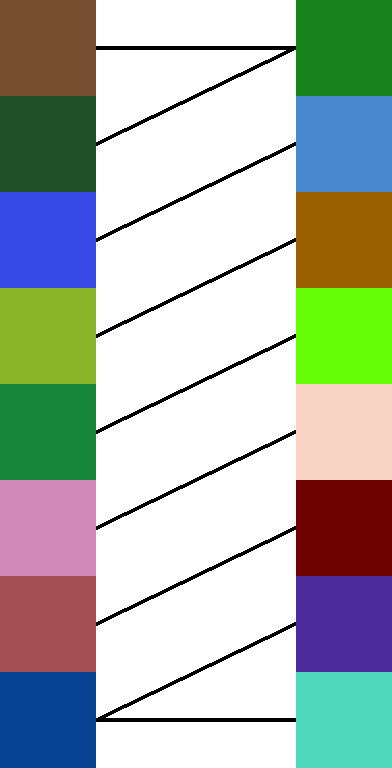
\includegraphics[width=0.30\linewidth]{img/dtw_ex2.png}
    \caption{Zuordnung der Pixel beim DTW-Algorithmus}
    \label{fig-dtw-ex2}
\end{figure}
Wie zu sehen ist, ist dieses Matching auch gültig, da jedes Element mindestens einen Partner hat und sich außerdem keine Verbindungen überkreuzen.
\section{Mahalanobis Gradient Compatibility (MGC)}\label{section-mgc}
Die Mahalanobis Gradient Compatibility (MGC) wurde zuerst in \cite{gallagher} beschrieben und später in weiteren Werken \cite{linear,paikin,loop,robust,crisjim} verwendet oder je nach Problemstellung leicht angepasst.

Bei dieser Art der Kompatibilität wird zunächst von allen vier Seiten jedes Puzzlestückes der durchschnittliche Wert der Ableitungen (vgl. \ref{section-pbc}) berechnet (für allen drei Farb-Channels). Mit diesen Ableitungen und dem Durchschnitt lässt sich dann die Kovarianzmatrix bezüglich diesen Ableitungen berechnen. Beim Vergleich zweier Puzzlestücke werden dann wieder beide Seiten betrachtet. Es wird zunächst die Mahalanobis-Distanz von allen Ableitungen zwischen den Puzzlestücken bezüglich der Verteilung von einem Puzzlestück berechnet und aufsummiert. Um die Symmetrie beizubehalten wird dies auch noch von der anderen Seite gemacht. Die Mahalanobis-Distanz berechnet dabei die (euklidische) Distanz eines Ableitungsvektors (mit drei Komponenten für die entsprechenden Channels) bezüglich eines Koordinatensystems welches durch den Durchschnittsvektor und der Kovarianzmatrix (des jeweils anderen Puzzlestückes) beschrieben wird. Der Durchschnittsvektor bildet dabei den Ursprung des Koordinatensystems und die (normierten) Eigenvektoren der Kovarianzmatrix bilden die Achsen. Die Mahalanobis-Distanz führt zunächst diese Koordinatentransformation durch, um danach die Distanz eines Vektors in diesem Koordinatensystem berechnen zu können.

Es werden im Folgenden wieder zwei Puzzlestücke $x_i$ und $x_j$ betrachtet, wobei $r=0$ und $x_i$ damit links von $x_j$ platziert wird. Die Distanz $D(x_i,x_j,r)$ wird wieder in zwei Teile aufgeteilt (ähnlich wie bei der PBC in \ref{section-pbc}): $D(x_i,x_j,r)=D_L(x_i,x_j,r)+D_R(x_i,x_j,r)$. Damit ist die Symmetrie der Distanz garantiert und es gilt $D(x_i,x_j,r)=D(x_i,x_j,r')$. Es wird im Folgenden dann nur die Berechnung für $D_L(x_i,x_j,0)$ aufgeführt. Für diese Berechnung ist es zunächst nötig, die Ableitungen von $x_i$ an der rechten Seite zu berechnen. Wie in \ref{section-pbc} wird dafür der Backward-Differenzenquotient entlang der x-Achse genommen. In der Literatur werden diese Ableitungen als Gradient $G$ bezeichnet. Für die rechte Seite von $x_i$ ergeben sich die Ableitungsvektoren dann folgendermaßen (es ist zu beachten, dass ein $G$ drei Komponenten hat):
\begin{align}\label{eq-mgc1}
    G_k=x_i(w-1,k)-x_i(w-2,k),\;\forall 0\leq k<h
\end{align}
Damit lässt sich dann der durchschnittliche Ableitungsvektor bestimmen:
\begin{align}\label{eq-mgc2}
    \mu=\frac{1}{h}\sum_{k=0}^{h-1}G_k
\end{align}
Mit allen Ableitungsvektoren und dem durchschnittlichen Ableitungsvektor lässt sich dann die Kovarianzmatrix $S$ bestimmen. Dies ist hier eine $3\times3$ Matrix und lässt sich folgendermaßen bestimmen:
\begin{align}\label{eq-mgc3}
    S=\frac{1}{h-1}\sum_{k=0}^{h-1}(G_k-\mu)(G_k-\mu)^\mathsf{T}
\end{align}
Um numerische Probleme bei der späteren Invertierung von $S$ zu vermeiden, lassen sich einige \textit{dummy} Gradienten mit in die Berechnung der Matrix $S$ einbeziehen. Dabei wurde sich an \cite{gallagher,crisjim} orientiert und es wurden neun solcher Gradienten gewählt. Diese Gradienten lauten
\begin{align*}
    &(0,0,0),(1,1,1),(-1,-1,-1),\\
    &(0,0,1),(0,1,0),(1,0,0),\\
    &(-1,0,0),(0,-1,0),(0,0,-1)
\end{align*}
Die Mahalanobis-Distanz von einem Vektor $x$ berechnet sich dann zu:
\begin{align}\label{eq-mgc4}
    D_M(x)=\sqrt{(x-\mu)^\mathsf{T}S^{-1}(x-\mu)}
\end{align}
Es ist nun möglich mit \ref{eq-mgc2}, \ref{eq-mgc3} und \ref{eq-mgc4} die einseitige Gesamtdistanz $D_L(x_i,x_j,0)$ zu definieren. Dabei ist lediglich zu beachten, dass nach \cite{gallagher} die Wurzeloperation aus \ref{eq-mgc4} weggelassen wird.
\begin{align}\label{eq-mgc5}
    D_L(x_i,x_j,0)=\sum_{k=0}^{h-1}(G_k^{i\rightarrow j}-\mu)^\mathsf{T}S^{-1}(G_k^{i\rightarrow j}-\mu)
\end{align}
Dabei ist $G_k^{i\rightarrow j}$ der Ableitungsvektor der beim Übergang von einem Puzzlestück zum anderen entsteht, wenn man die beiden Puzzlestücke $x_i$ und $x_j$ nun (mit $x_i$ links von $x_j$) zusammenfügt. Dafür gilt:
\begin{align}\label{eq-mgc6}
    G_k^{i\rightarrow j}=x_j(0,k)-x_i(w-1,k),\;\forall 0\leq k<h
\end{align}
Bezüglich der Implementation lässt sich sagen, dass es durchaus möglich ist (ähnlich wie in \ref{section-pbc}), die Ableitungsvektoren, den durchschnittlichen Ableitungsvektor und auch die Inverse der Kovarianzmatrix (es wird zu jederzeit nur die Inverse von $S$ benötigt, daher lohnt es sich nicht auch $S$ selber abzuspeichern) jeder Seite (und für jedes Puzzlestück) nur einmal zu berechnen und diese dann abzuspeichern. Bei dem eigentlichen Vergleich zweier Puzzlestücke müssen dann nur \ref{eq-mgc5} und \ref{eq-mgc6} berechnet werden. Trotz der großen Anzahl und höheren Komplexität der Berechnungen, ist das Laufzeitverhalten der kompletten Prozedur linear in der Länge der Kante (beispielsweise $h$ wie in den obigen Gleichungen). Berechnungen wie \ref{eq-mgc3} oder \ref{eq-mgc5} haben aufgrund der Matrizenmultiplikationen zwar größeren konstanten Aufwand (in der Summe), da jede Matrix aber die Dimensionen $1\times3$, $3\times1$ oder $3\times3$ besitzt, sind die Dimensionen der Matrizen und somit auch alle Operationen mit diesen Matrizen konstant.

Diese Linearität dieses Verfahrens bietet einen großen Vorteil bei der Berechnung von sehr hochauflösenden Bildern (bzw. hochauflösenden Puzzlestücken). Verfahren wie etwa DTW (\ref{section-dtw}) sind dort aufgrund der quadratischen Laufzeit eher weniger geeignet. Diese Tatsache und ein komplexeres Verfahren zur Bewertung der Übergänge zwischen zwei Puzzlestücken (im Vergleich zu der trivialeren PBC in \ref{section-pbc}), hat dazu geführt, dass selbst komplexere Jigsaw-Puzzle-Solver (wie etwa \cite{paikin}) noch diese Metrik verwenden. Aus diesen Gründen wurde diese Metrik auch für den folgenden Algorithmus verwendet.
\chapter{Algorithmus zur Puzzle-Assemblierung}
Ausgestattet mit einer Vielzahl von Metriken aus \ref{ch-metrics} gilt es nun einen Algorithmus zu entwickeln, der die eigentliche Assemblierung des Puzzles übernimmt. Dabei wird aktuell noch von einem Jigsaw-Puzzle ausgegangen bei dem keine Puzzlestücke fehlen (bei Schiebepuzzles fehlt entsprechend ein Stück, auf diesen Sonderfall wird dort eingegangen, wo dieser Fall Probleme beim Algorithmus bereitet). Da das Jigsaw-Puzzle nachweisbar als NP-Hard gilt \cite{dem}, beruhen alle bekannten algorithmischen Puzzle-Löser auf einen heuristischen Ansatz, um große Puzzle lösen zu können.

Aktuelle Methoden zum Lösen von Jigsaw-Puzzles lassen sich grob in zwei Kategorien aufteilen:
\begin{enumerate}
    \item Greedy Methoden \cite{loop,pomeranz,gallagher}, welche probieren aus den paarweisen Distanzen der einzelnen Puzzlestücke iterativ ein Gesamtbild zu assemblieren, indem in jedem Schritt die günstigsten bzw. besten Puzzlestücke miteinander verbunden werden.
    \item Globale Methoden, welche probieren eine globale Kompatibilitätsfunktion zu maximieren (bzw. eine globale Distanzfunktion zu minimieren) um dabei ein globales Maximum (oder Minimum im Falle einer Distanzfunktion) zu finden. Darunter fallen unter anderem Ansätze aus der genetischen Programmierung \cite{genetic}, linearen Programmierung \cite{linear} und auch probabilistische Verfahren \cite{cho}.
\end{enumerate}
In dieser Arbeit wird sich auf das Spannbaum Verfahren von Gallagher \cite{gallagher} fokussiert. Dieses Verfahren lässt sich in die Kategorie der Greedy Methoden einordnen und basiert hauptsächlich auf der Observierung, dass gängige Algorithmen zur Berechnung eines minimalen Spannbaums (Minimum Spanning Tree - MST) mit wenigen Änderungen bereits in der Lage dazu sind, simple Jigsaw-Puzzle zu assemblieren. Diese Idee wurde dann so perfektioniert, dass Gallagher selber in der Lage dazu war, Puzzle mit mehreren tausend Puzzlestücken perfekt zu rekonstruieren. Neben dieser vielversprechenden Ergebnisse und der Tatsache, dass dieses Verfahren auch das erste Verfahren war, welches die MGC (vgl. \ref{section-mgc}) verwendet hat (auch diese wurde von Gallagher selber in \cite{gallagher} beschrieben), basiert dieses Verfahren trotz State-of-the-Art Ergebnisse hauptsächlich auf Methoden der Graphentheorie. Andere Verfahren mit vergleichbaren Ergebnissen (etwa das probabilistische Verfahren von Cho et al. \cite{cho}) basieren auf tiefliegendere und komplexere stochastische Zusammenhänge.

Neben dem Algorithmus selber und einige Änderungen um diesen auch für Schiebepuzzle möglich zu machen, wird außerdem eine effiziente Datenstruktur beschrieben, auf die der Algorithmus arbeiten wird. Dabei handelt es sich um eine modifizierte Version der Disjoint-Set-Datenstruktur oder auch Disjoint-Set-Forest.\cite{dsf} Bei den Anforderungen dieser Datenstruktur wird sich sowohl an Gallagher selber gerichtet \cite{gallagher}, als auch an C. Zanoci und J. Andress Beschreibung von Gallaghers Algorithmus.\cite{crisjim}
\section{Baum-basierte Assemblierung nach Gallagher}
Es wird das Jigsaw-Puzzle Problem als Graph $G=(V,E)$ betrachtet mit der Menge der Puzzlestücke als Vertices $V$ und die Menge der möglichen Verbindungen von zwei Puzzlestücken als Kanten $E$. Diese Kanten sind gewichtet und erhalten ihre Kantengewichte nach einer der in Kapitel \ref{ch-metrics} vorgestellten Metriken (vorzugsweise die MGC). Außerdem sei zu beachten, dass zwei Puzzlestücken nicht nur durch eine Kante sondern durch exakt vier Kanten in Verbindung stehen - jeweils eine für jede mögliche räumliche Anordnung der beiden Puzzleteile (vgl. Tabelle \ref{tbl-spatial-relation}).

Da das fertige Puzzle eine Zusammenhangskomponente des Graphen darstellt (und zwar eine mit minimaler oder nahezu minimaler Kantengewichtssumme), bietet sich ein Algorithmus zur Berechnung des minimalen Spannbaums an. Ein solcher Algorithmus wäre in der Lage eine solche minimale Zusammenhangskomponente zu finden. Der minimale Spannbaum der durch einen solchen Algorithmus entstehen würde stellt in aller Regel jedoch keine legale Puzzlestellung dar. Dazu muss zusätzlich noch sichergestellt werden, dass jederzeit keine zwei Puzzlestücke in der Zusammenhangskomponente übereinander liegen. Diese zusätzliche Einschränkung des Algorithmus ist eine weitere Motivation für die Implementation einer modifizierten Disjoint-Set-Datenstruktur, die den räumlichen Zusammenhang der Zusammenhangskomponenten kennt und vermeidet, dass Zusammenhangskomponenten zusammengeführt werden, welche zu übereinander liegenden Puzzlestücken führen würden.

Entsprechend solch einer Datenstruktur wird damit im Zusammenhang der Algorithmus von Kruskal \cite{kruskal} betrachtet, um den minimalen Spannbaum in einem Graphen zu finden. Dabei werden am Anfang des Algorithmus alle Vertices (die Puzzlestücke) zunächst als seperate Zusammenhangskomponenten aufgefasst. Damit bildet jeder Vertex einen Baum, die Menge aller Bäume wird als Wald (Forest) bezeichnet. Daraufhin werden die Kanten des Graphen in absteigender Reihenfolge (bezüglich des Kantengewichts) betrachtet. Verbindet eine Kante zwei Vertices, welche sich bereits in der selben Zusammenhangskomponente befinden, so wird diese Kante nicht zum Baum hinzugefügt, da diese dort sonst eine Schleife erzeugen würde. Im Falle wo diese Kante zwei Vertices verbinden würde, welche sich in verschiedenen Zusammenhangskomponenten befinden, so wird diese Kante zum Baum hinzugefügt. Dieser Schritt verbindet die beiden Zusammenhangskomponenten zu einer größeren Zusammenhangskomponente. Dieser Vorgang wird solange wiederholt, wie noch Kanten vorhanden sind und es sich noch kein Spannbaum gebildet hat (es existieren noch mindestens zwei seperate Bäume im Wald).

Die normale Disjoint-Set-Datenstruktur (Disjoint-Set-Forest) \cite{dsf} übernimmt dabei die Aufgabe, die Menge der Vertices $V$ in disjunkte zusammenhängende Mengen (Zusammenhangskomponenten) zu partitionieren. Die üblichen Operationen auf eine solche Datenstruktur sind unter anderem das Initialisieren eines solchen disjunkten Waldes mit $n$ Elementen (was in $\Theta(n)$ Zeit möglich ist), das Testen, ob zwei Elemente sich in der selben Menge befinden und das Vereinigen zweier Mengen.

Die Laufzeit der letzten beiden Operationen hängt stark von der Implementation der Datenstruktur ab. Bei einer guten Implementation sind beide Operationen durchschnittlich $\Theta(\alpha(n))$.\cite{dsf-log,dsf-lower,tarjan,tarjan2,tarjan3} Wobei $\alpha(n)$ für die inverse Funktion der eindimensionalen Ackermann-Funktion $f(n)=A(n,n)$ steht. Die Funktion $f(n)$ nimmt bereits für kleine $n$ sehr große Werte an. So ist bereits $f(4)=A(4,4)=2\uparrow\uparrow7-3$ in Knuth's \textit{uparrow} Notation. Als Potenz ergibt sich der \textit{Power-Tower} $f(4)=2^{2^{2^{2^{2^{2^2}}}}}-3$. Die einfachste Potenz die dies noch darstellen kann ist $f(4)=2^{2^{2^{65536}}}-3$. Selbst die innerste Potenz $2^{65536}$ ist bereits unvorstellbar groß. Dementsprechend lässt sich sagen, dass die inverse Ackermann-Funktion selbst für sehr große $n$ stets Werte annehmen wird, die $4$ nicht überschreiten. Damit lässt sich sagen, dass Operationen mit einem Laufzeitverhalten von $\Theta(\alpha(n))$ \textit{quasi konstant} sind.

Ein Disjoint-Set-Forest (DSF) wird in der Regel als kompaktes Array implementiert. Jedes Element im Array ist dann ein Element im Forest (also ein Element eines Baums im Wald). Die Array-Indizes können dann dazu dienen die Elemente zu identifizieren. Jedes Element enthält dann zusätzlich noch einen Parent-Pointer (bei Arrays bietet sich auch ein Parent-Index an). Um zwei Mengen später effizient vereinigen zu können, lässt sich auch noch ein zusätzliches Feld definieren, welches die Anzahl der Elemente mitspeichert, die sich in dem selben Baum wie das Element befinden. Dieses Feld ist nur für Elemente von Bedeutung, die die Wurzel ihres Baumes darstellen (da nur dort die Anzahl erhöht wird). Die Beziehungen der Elemente über den Parent-Index bilden einen \textit{rückverweisenden} Baum: Es lässt sich bei jedem beliebigen Element starten und solange der Parent-Index verfolgen, bis dieser entweder ungültig (\texttt{null}) ist oder (bei Arrays üblich) ein Element der Parent von sich selber ist. Dieses Element ist die Wurzel des Baums, der alle Elemente enthält, die dieses Element auch als Wurzel haben. Dieses Wurzelelement \textit{repräsentiert} seine Menge.

Die \texttt{InitForest} Operation initialisiert einen DSF mit einer vorgegeben Kapazität $n$. Jedes Element befindet sich anfangs in seiner eigenen Menge.
\begin{algorithm}[H]
    \caption{Initialisierung eines Disjoint-Set-Forest}\label{alg-dsf-init}
    \begin{algorithmic}
        \Procedure{InitForest}{$n$}
            \State nodes $\gets$ array$[n]$
            \For{$i=1$ to $n$}
                \State nodes$[i]$.parent $\gets i$\Comment{Element ist Wurzel seiner Menge}
                \State nodes$[i]$.size $\gets 1$\Comment{Menge enthält nur dieses Element}
            \EndFor
        \EndProcedure
    \end{algorithmic}
\end{algorithm}
Die FindRoot Operation übernimmt ein Element $x$ und gibt den Index des Wurzelelementes der Menge zurück in der sich $x$ befindet.
\begin{algorithm}[H]
    \caption{FindRoot Operation mit Pfadkomprimierung}\label{alg-dsf-find}
    \begin{algorithmic}
        \Function{FindRoot}{$x$}
            \If{$x$.parent $\neq x$}
                \State $x$.parent $\gets$ FindRoot($x$.parent)
            \EndIf
            \State \Return $x$.parent
        \EndFunction
    \end{algorithmic}
\end{algorithm}

\backmatter

\preparebibliography
\bibliography{bibliography}

\end{document}